\documentclass[11pt,a4paper]{article}
\usepackage[margin=2.5cm]{geometry}
\usepackage{subcaption}
\usepackage{amsmath}
\usepackage{graphicx}
\usepackage{booktabs}
\usepackage{float}
\usepackage{hyperref}
% Improved academic report formatting
\usepackage{lmodern}
\usepackage{microtype}
\usepackage{setspace}
\usepackage{titlesec}
\titlespacing{\section}{0pt}{12pt}{2pt}
\titlespacing{\subsection}{0pt}{6pt}{4pt}
\setstretch{1.12}
\setlength{\parindent}{0pt}
\setlength{\parskip}{6pt}
\setlength{\abovedisplayskip}{6pt}
\setlength{\belowdisplayskip}{6pt}
\title{Exploratory Statistical Analysis of
Amazon Data Science Books}
\author{
Florentia Pattidou \and
Valeria Shirshina \and
Marios Makrygiannis
}
\date{University of Cyprus\
DSC531 -- Statistical Simulation and Analysis}
\begin{document}
\maketitle
ewpage
\begin{abstract}
This report presents an exploratory statistical analysis of the Amazon Data Science Books dataset using the R programming language. The objective is to examine the characteristics of data science books, assess data quality, summarize key numerical variables, and investigate relationships between book attributes and customer reviews.
The original dataset contains 946 observations and 11 variables. During data cleaning, one duplicate observation was removed, missing values were examined, and book weights were converted into kilograms. Potential outliers were investigated using the interquartile range (IQR) method and additional weight-per-page checks. Ten potentially suspicious weight measurements were flagged for a separate sensitivity analysis without removing the corresponding books.
Descriptive statistics and graphical methods were used to explore the distributions of prices, page counts, ratings, review counts, and weights. The results indicate that review counts are highly right-skewed, while average customer ratings are generally concentrated toward the upper end of the rating scale. A moderate positive correlation was observed between page counts and prices (r = 0.444).
Overall, the analysis demonstrates how data cleaning, descriptive statistics, and visualization can support the interpretation of real-world book data.
\end{abstract}
ewpage
\tableofcontents
ewpage
\section{Introduction}
Data analysis plays an important role in understanding patterns, identifying relationships, and extracting meaningful insights from real-world datasets. Statistical methods allow researchers to summarize large amounts of information, evaluate variability, and investigate potential associations between variables.
This report presents an exploratory statistical analysis of the Amazon Data Science Books dataset using the R programming language. The dataset contains information about books related to data science, including their prices, number of pages, average customer ratings, number of reviews, rating distributions, and physical weights.
The primary objective of this study is to examine the characteristics of the dataset through data cleaning, descriptive statistics, and graphical visualization. Particular attention is given to identifying missing values, duplicate observations, potentially unusual measurements, and patterns within the numerical variables.
Additionally, the analysis investigates relationships between selected book characteristics, such as the association between the number of pages and price, the relationship between pages and physical weight, and the connection between customer ratings and review counts.
By combining statistical summaries with visual representations, this study aims to provide a clearer understanding of the dataset and demonstrate how exploratory data analysis can support informed interpretation of real-world information.
\section{Dataset Description}
\subsection{Dataset Overview}
The Amazon Data Science Books dataset contains 946 observations
and 11 variables describing book characteristics and customer
feedback. These include prices, page counts, customer ratings,
review counts, star-rating proportions, weights, and languages.
The dataset was imported into R using \texttt{read.csv()}
and initially examined using \texttt{dim()}, \texttt{str()},
and \texttt{summary()}. This examination identified missing
values and inconsistent weight units, which were addressed
during data cleaning.
\subsection{Description of Variables}
Table~\ref{tab:variables} presents the variables included
in the original dataset, their data types, and their meanings.
\begin{table}[H]
\centering
\small
\begin{tabular}{lll}
\toprule
Variable & Data Type & Description \
\midrule
\texttt{price} & Numeric & Book price \
\texttt{pages} & Integer & Number of pages \
\texttt{avg_reviews} & Numeric & Average customer rating (1--5) \
\texttt{n_reviews} & Integer & Number of customer reviews \
\texttt{star5} & Numeric & Proportion of five-star ratings \
\texttt{star4} & Numeric & Proportion of four-star ratings \
\texttt{star3} & Numeric & Proportion of three-star ratings \
\texttt{star2} & Numeric & Proportion of two-star ratings \
\texttt{star1} & Numeric & Proportion of one-star ratings \
\texttt{weight} & Character & Book weight in ounces or pounds \
\texttt{language} & Character & Language of the book \
\bottomrule
\end{tabular}
\caption{Description of the Original Dataset Variables}
\label{tab:variables}
\end{table}
The five star-rating variables represent proportions rather
than absolute review counts. The weight variable requires
conversion to a common measurement unit before numerical analysis.
\subsection{Initial Data Quality Assessment}
Table~\ref{tab:missing} summarizes the missing values
identified during the initial inspection of the dataset.
\begin{table}[H]
\centering
\begin{tabular}{lr}
\toprule
Variable & Missing Values \
\midrule
\texttt{price} & 2 \
\texttt{pages} & 12 \
\texttt{avg_reviews} & 123 \
\texttt{weight} & 3 blank strings \
\texttt{language} & 3 blank strings \
\bottomrule
\end{tabular}
\caption{Initial Missing Values}
\label{tab:missing}
\end{table}
The initial assessment identified missing information
in several variables. Blank strings in the weight and
language fields required conversion to \texttt{NA}.
Missing observations were not automatically removed,
allowing available information to be retained for
subsequent analysis. Duplicate records and potentially
unusual measurements were investigated during the
cleaning process described in Section~\ref{sec:cleaning}.
\section{Data Cleaning}
\label{sec:cleaning}
\subsection{Data Cleaning Overview}
Data cleaning was performed in R to improve data consistency
while preserving as much information as possible. The procedures
included handling missing values, removing duplicate observations,
standardizing weight measurements, investigating outliers,
and validating customer review information.
\subsection{Missing Values and Duplicate Observations}
Blank strings in the weight and language variables were converted
to \texttt{NA}. Missing values were handled using available-case
calculations rather than deleting incomplete observations.
One exact duplicate was identified and removed, reducing the
dataset from 946 to 945 observations.
\subsection{Weight Standardization}
Book weights were originally recorded in two units:
ounces (204 observations) and pounds (738 observations),
with 3 missing measurements.
The following conversion factors were applied:
\begin{align}
\text{Ounces to kilograms:}\quad
W_{\mathrm{kg}} &= W_{\mathrm{oz}} \times 0.0283495 \[8pt]
\text{Pounds to kilograms:}\quad
W_{\mathrm{kg}} &= W_{\mathrm{lb}} \times 0.4535924
\end{align}
\subsection{Outlier Detection Using the IQR Method}
Potential outliers were identified using the interquartile
range (IQR) method, with boundaries defined as:
\begin{align}
IQR &= Q_3 - Q_1 \[6pt]
\text{Lower Bound} &= Q_1 - 1.5 \times IQR \[6pt]
\text{Upper Bound} &= Q_3 + 1.5 \times IQR
\end{align}
For book weight, the IQR was approximately 0.448 kg, producing an upper boundary of 1.602 kg. The method identified 41 potential weight outliers. Other variables also contained outliers: price (97), pages (17), average ratings (34), and review counts (111).
These observations were not automatically removed because extreme values may represent genuine book characteristics rather than recording errors.
\subsection{Investigation of Suspicious Weight Measurements}
The IQR method identified potential weight outliers, but
these observations were not necessarily incorrect. To
investigate unusual weight measurements further, the
relationship between book weight and page count was examined.
A weight-per-page ratio was calculated for books with
available positive page counts and weight measurements:
[
\text{Weight per page (g/page)}
=
\frac{1000 \times W_{\mathrm{kg}}}{\text{Pages}}
]
Measurements outside the exploratory range of
0.3--10 grams per page were flagged as potentially
suspicious. This criterion identified 10 observations.
\begin{table}[H]
\centering
\begin{tabular}{ll}
\toprule
Criterion & Value \
\midrule
Lower threshold & 0.3 g/page \
Upper threshold & 10 g/page \
Flagged observations & 10 \
\bottomrule
\end{tabular}
\caption{Criteria for Flagging Suspicious Weight Measurements}
\label{tab:weightcriteria}
\end{table}
The flagged measurements were not confirmed data errors.
Therefore, the corresponding books were retained in the
cleaned dataset. For weight-specific sensitivity analysis,
a separate variable, \texttt{weight_analysis}, was created
by replacing the 10 flagged weight values with \texttt{NA}.
The mean weight decreased from approximately 0.778 kg to
0.753 kg, while the standard deviation decreased from
0.583 kg to 0.404 kg. The Pearson correlation between
page count and weight increased from 0.571 to 0.865.
Because the filtering criterion was based on weight
relative to page count, this increase should be
interpreted cautiously rather than as independent
evidence of a stronger underlying relationship. The corresponding scatterplots are presented in Figure~\ref{fig:pagesweight}.
\begin{figure}[H]
\centering
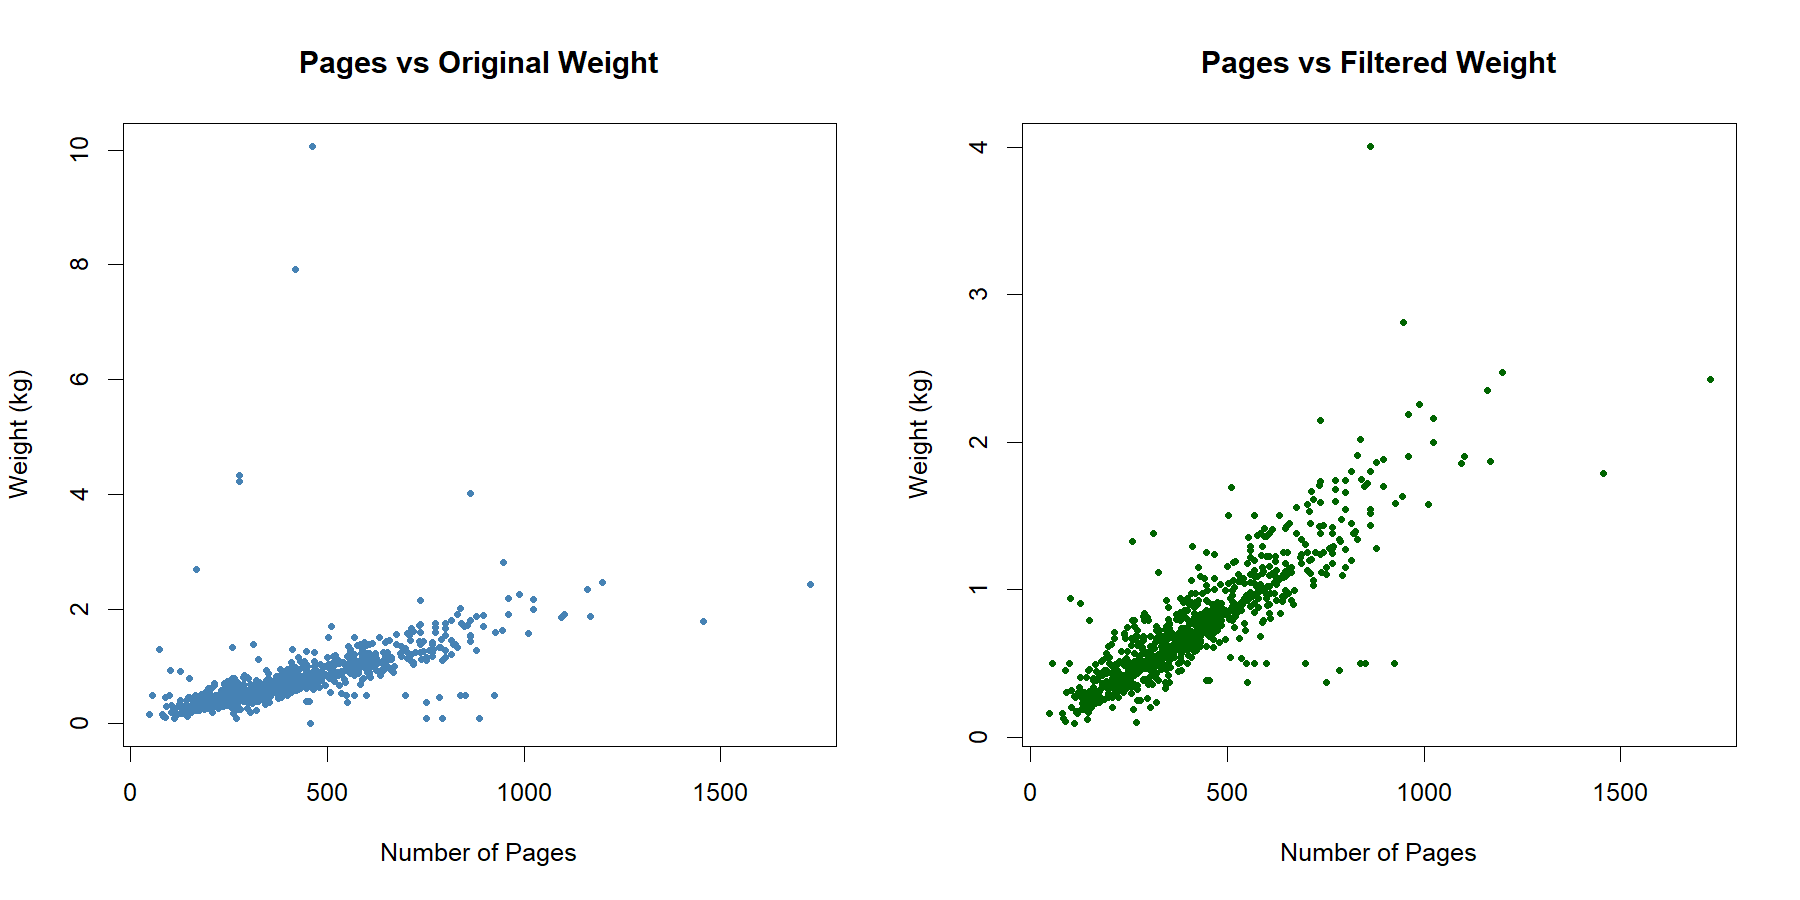
\includegraphics[width=0.85\textwidth]{plots/4_6_pages_vs_weight.png}
\caption{Relationship Between Page Count and Book Weight Before and After Filtering Suspicious Measurements}
\label{fig:pagesweight}
\end{figure}
\subsection{Review Data Consistency}
Customer review information was examined to identify
inconsistencies between review counts, average ratings,
and star-rating proportions.
A total of 123 books had zero customer reviews. For
these observations, the star-rating proportions were
set to \texttt{NA}, since no rating distribution could
be meaningfully calculated.
For the remaining 822 books with customer reviews,
the five star-rating proportions were checked to
determine whether their sum was approximately equal
to one. No observations exceeded a tolerance of
0.05 from the expected total.
These checks helped ensure that the review-related
variables were internally consistent before
subsequent statistical analysis.
\subsection{Final Cleaned Dataset}
After data cleaning, the dataset contained 945 observations,
following the removal of one exact duplicate. Missing values
were preserved as \texttt{NA}, and available weight measurements
were standardized to kilograms.
The cleaned dataset included the original numerical book
characteristics and star-rating proportions, together with
two weight-related variables: \texttt{weight_kg}, containing
the standardized measurements, and \texttt{weight_analysis},
used for sensitivity analysis after flagging 10 potentially
suspicious weight values.
\begin{table}[H]
\centering
\begin{tabular}{ll}
\toprule
Characteristic & Final Result \
\midrule
Original observations & 946 \
Final observations & 945 \
Duplicate observations removed & 1 \
Available weight measurements & 942 \
Weight values used in sensitivity analysis & 932 \
Flagged suspicious weights & 10 \
\bottomrule
\end{tabular}
\caption{Summary of the Final Cleaned Dataset}
\label{tab:cleaned}
\end{table}
The cleaned dataset was exported as a CSV file for
subsequent descriptive statistics and visualization.
No books were removed solely because of extreme values
or missing information.
\section{Descriptive Statistics}
\subsection{Summary of Numerical Variables}
Descriptive statistics were calculated for the main numerical
variables, including book prices, page counts, average customer
ratings, review counts, and filtered book weights.
Table~\ref{tab:descriptive} presents the number of available
observations, mean, median, standard deviation, coefficient
of variation (CV), and skewness.
\begin{table}[H]
\centering
\small
\begin{tabular}{lrrrrrr}
\toprule
Variable & N & Mean & Median & SD & CV (%) & Skewness \
\midrule
Price & 943 & 52.111 & 43.970 & 36.609 & 70.25 & 2.421 \
Pages & 933 & 419.478 & 384.000 & 204.060 & 48.65 & 1.123 \
Average Rating & 822 & 4.441 & 4.500 & 0.401 & 9.03 & -2.011 \
Number of Reviews & 945 & 137.898 & 25.000 & 499.731 & 362.39 & 9.467 \
Filtered Weight (kg) & 932 & 0.753 & 0.669 & 0.404 & 53.66 & 1.670 \
\bottomrule
\end{tabular}
\caption{Descriptive Statistics of the Main Numerical Variables}
\label{tab:descriptive}
\end{table}
The number of available observations differs between variables
because missing values were excluded only from the relevant
calculations. Filtered weight statistics were calculated using
the \texttt{weight_analysis} variable.
\subsection{Central Tendency and Variability}
The number of customer reviews exhibits the greatest relative
variability (CV = 362.39%). Its mean (137.898) is considerably
higher than its median (25), indicating that a small number of
highly reviewed books influence the average.
Book prices also exhibit substantial variability (CV = 70.25%),
while page counts and filtered weights show moderate-to-high
relative variability. In contrast, average customer ratings
have the lowest CV (9.03%), indicating that ratings are
concentrated within a relatively narrow range.
\subsection{Distribution Shape and Skewness}
Skewness measures the asymmetry of a distribution.
Positive values indicate a longer right tail, while
negative values indicate a longer left tail.
Customer review counts exhibit strong positive skewness
(9.467), indicating that most books receive relatively
few reviews, while a small number receive exceptionally
high counts. Book prices (2.421), page counts (1.123),
and filtered weights (1.670) are also positively skewed.
In contrast, average customer ratings are negatively
skewed (-2.011), reflecting the concentration of ratings
toward the upper end of the five-star scale.
Original book weights had a skewness of 7.209, which
decreased to 1.670 after excluding ten potentially
suspicious measurements from the weight-specific analysis.
Overall, the distributions are asymmetric, highlighting
the importance of using the median and interquartile range
alongside the mean and standard deviation.
\section{Data Visualization}
\subsection{Histograms of Numerical Variables}
Histograms were used to examine the distributions of book
prices, page counts, customer review counts, average ratings,
and filtered book weights.
Figure~\ref{fig:histograms} presents the distributions of
these five numerical variables.
\begin{figure}[H]
\centering
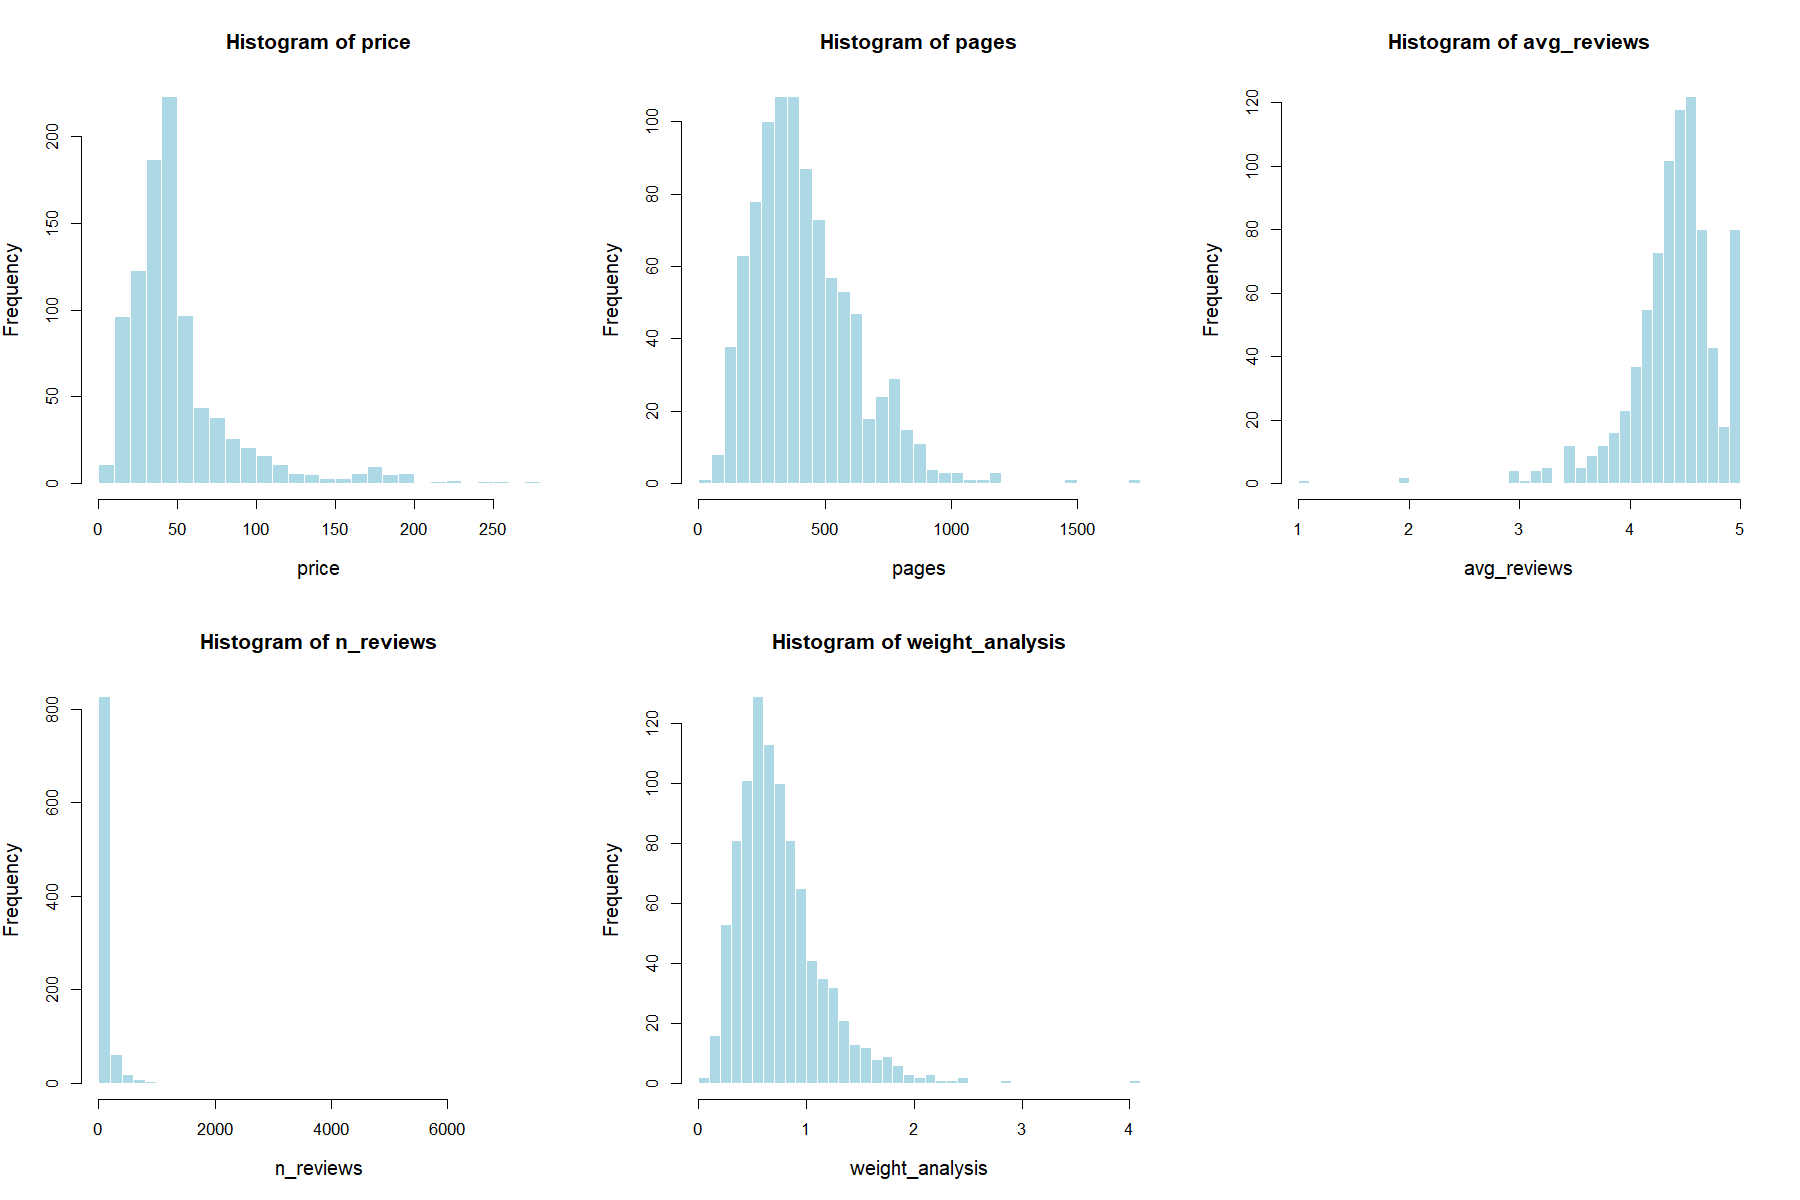
\includegraphics[width=0.95\textwidth]{plots/4_1_histograms.png}
\caption{Histograms of the Main Numerical Variables}
\label{fig:histograms}
\end{figure}
The histograms show that book prices, page counts, and
review counts are positively skewed. Review counts exhibit
particularly strong right-skewness, with most books receiving
relatively few reviews and a small number receiving thousands.
Average customer ratings are concentrated toward the upper
end of the five-star scale, while filtered book weights
remain positively skewed. These findings are consistent
with the descriptive statistics presented in Section 4.
\subsection{Boxplots and Outlier Visualization}
Boxplots were used to compare the variability of the main
numerical variables and identify observations lying beyond
the typical range of each distribution.
Figure~\ref{fig:boxplots} presents the boxplots of book
prices, page counts, average ratings, review counts,
and filtered book weights.
\begin{figure}[H]
\centering
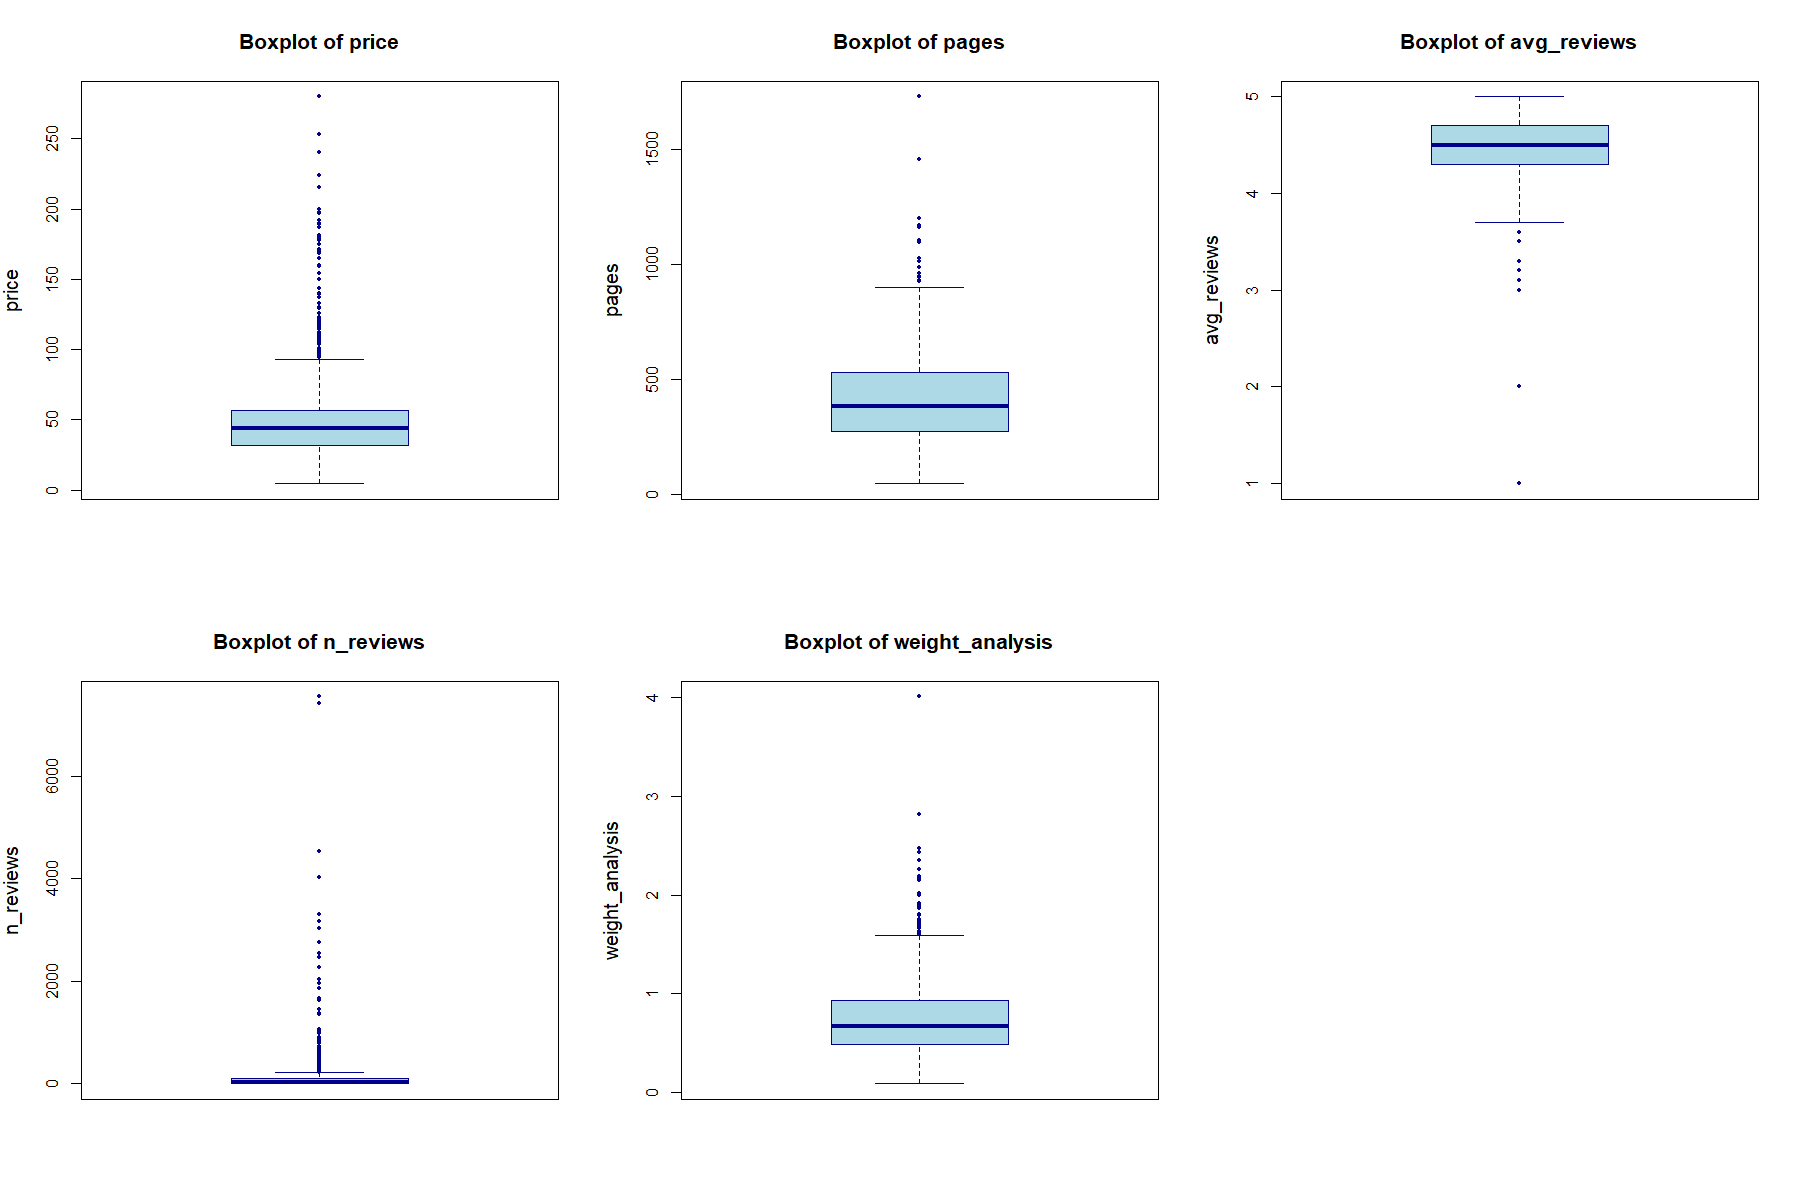
\includegraphics[width=0.95\textwidth]{plots/4_2_boxplots.png}
\caption{Boxplots of the Main Numerical Variables}
\label{fig:boxplots}
\end{figure}
The boxplots reveal substantial differences in the spread
of the numerical variables. Review counts exhibit numerous
extreme observations, consistent with their high standard
deviation and coefficient of variation.
Book prices and page counts also contain observations
beyond the upper whiskers, indicating the presence of
relatively expensive and unusually long books.
Average customer ratings are concentrated near the upper
end of the rating scale, with some comparatively low
ratings appearing as outliers. Filtered book weights
still contain high values, even after the ten suspicious
measurements were excluded from the weight-specific analysis.
Overall, these visualizations complement the descriptive
statistics and demonstrate that extreme observations
remain an important characteristic of the dataset.
\subsection{Log Transformation of Review Counts}
The number of customer reviews exhibited substantial
positive skewness, with a small number of books receiving
exceptionally high review counts.
To examine this distribution more clearly, a logarithmic
transformation was applied:
[
Y = \log(1 + X)
]
where $X$ represents the original number of reviews.
Adding one allows books with zero reviews to be included,
since $\log(0)$ is undefined.
Figure~\ref{fig:logreviews} compares the original and
log-transformed distributions.
\begin{figure}[H]
\centering
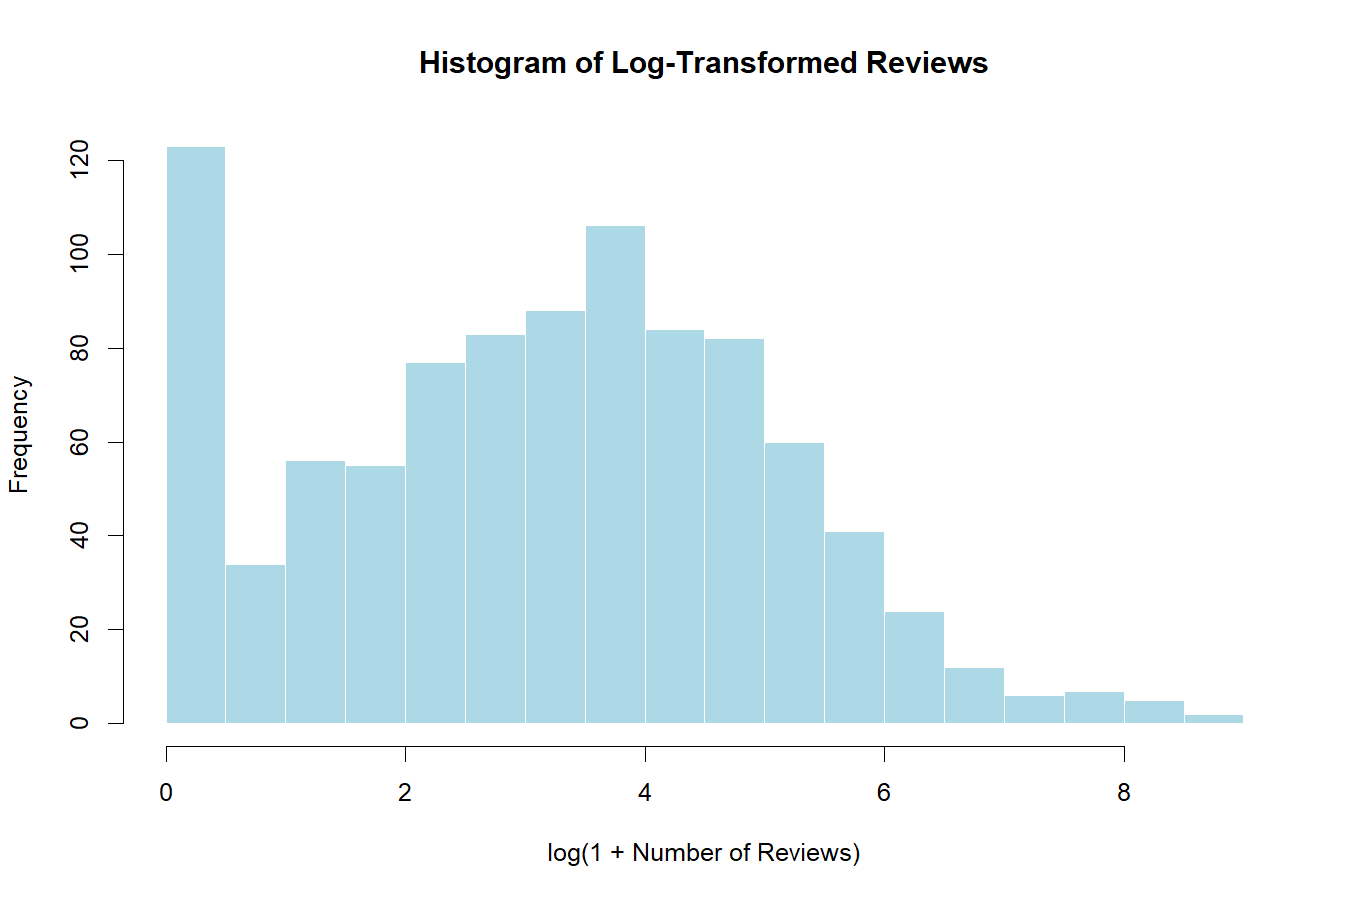
\includegraphics[width=0.85\textwidth]{plots/4_3_log_reviews.png}
\caption{Histogram of Log-Transformed Review Counts.}
\label{fig:logreviews}
\end{figure}
The original review-count distribution had a skewness
of 9.467, indicating a strong right tail. Following
the transformation, skewness decreased to approximately
0.055, indicating substantially reduced asymmetry.
The transformation compresses large review counts while
preserving their relative ordering. This makes the
distribution easier to visualize and may be useful for
subsequent statistical analysis. However, low skewness
alone does not establish that the transformed data
follow a normal distribution.
\subsection{Scatterplots and Relationships}
Scatterplots were used to visually examine relationships
between numerical variables.
Figure~\ref{fig:pagesprice} illustrates the relationship
between the number of pages and book price.
\begin{figure}[H]
\centering
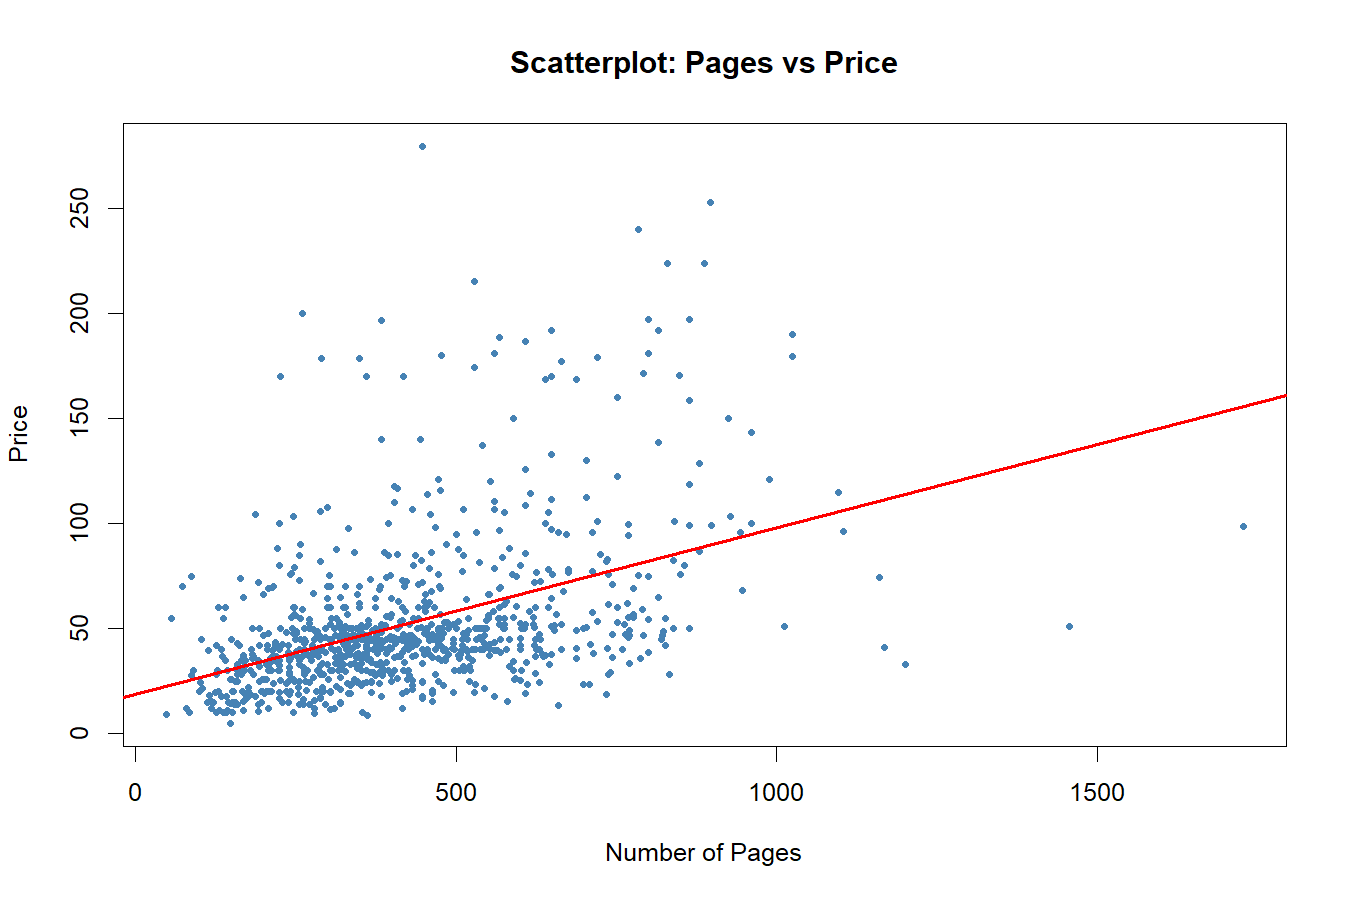
\includegraphics[width=0.85\textwidth]{plots/4_5_pages_vs_price.png}
\caption{Relationship Between Page Count and Book Price}
\label{fig:pagesprice}
\end{figure}
The scatterplot indicates a moderate positive relationship
between page count and price, with a Pearson correlation
coefficient of approximately 0.444.
This suggests that books with more pages tend to be more
expensive. However, considerable variation in price remains
among books with similar page counts.
The observed association does not imply that increasing
the number of pages directly causes a higher price.
\subsection{Customer Reviews and Ratings}
A scatterplot was also used to examine the relationship
between average customer ratings and the number of reviews.
Since review counts are highly right-skewed, the
log-transformed number of reviews was used to improve
the visualization.
Figure~\ref{fig:reviewsrating} illustrates the relationship
between average rating and log-transformed review counts.
\begin{figure}[H]
\centering
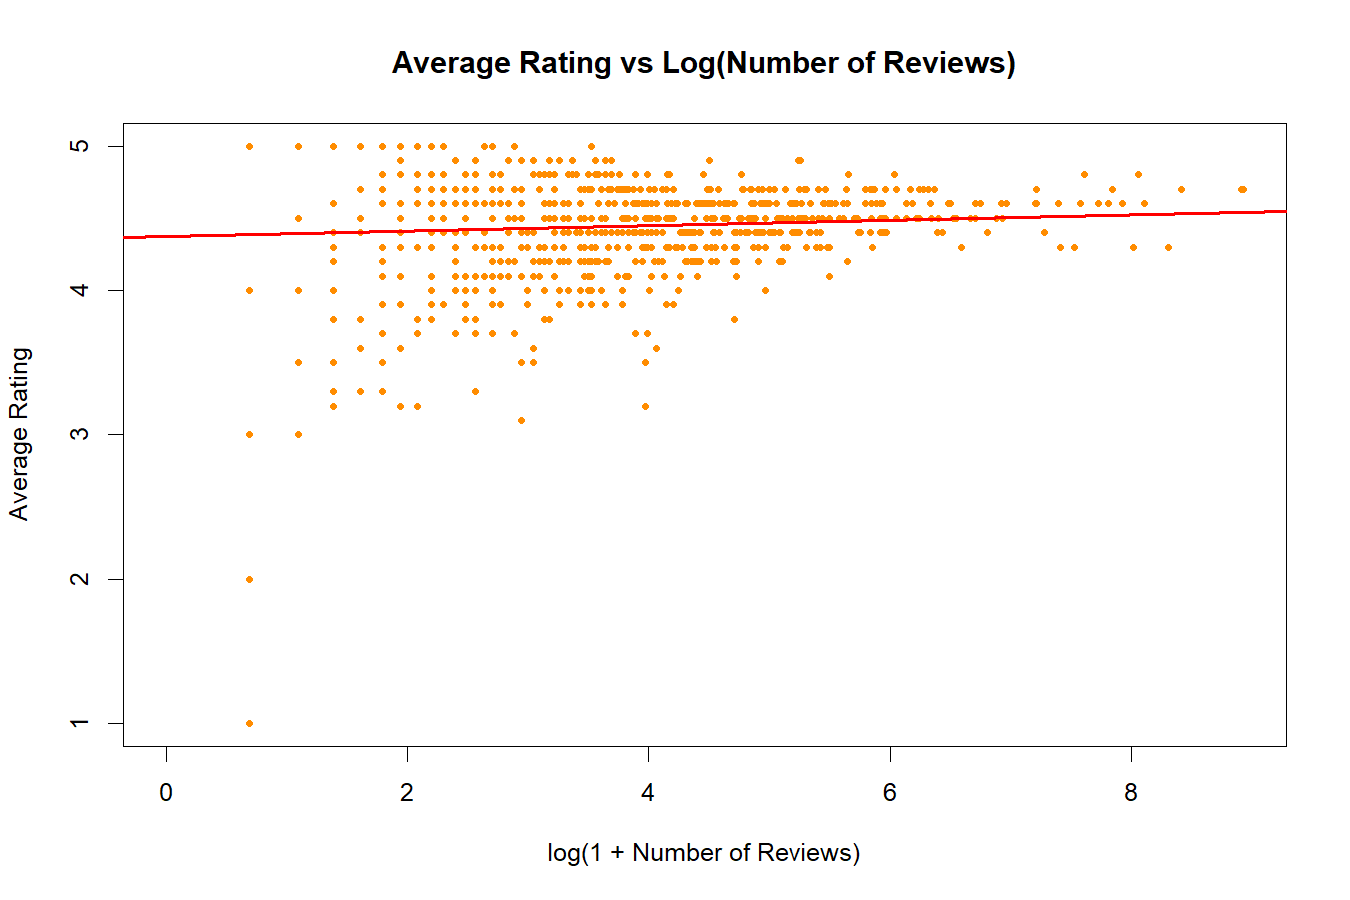
\includegraphics[width=0.85\textwidth]{plots/4_7_reviews_vs_rating.png}
\caption{Relationship Between Average Rating and
Log-Transformed Review Counts}
\label{fig:reviewsrating}
\end{figure}
The Pearson correlation coefficient between average rating
and log-transformed review counts was approximately 0.074,
indicating a very weak positive linear relationship.
The scatterplot suggests that books receiving more reviews
do not necessarily have higher average ratings. Books with
similar review counts may have substantially different
ratings.
Overall, the number of reviews appears to have little
linear association with the average customer rating
in this dataset.

---------------------------NEW-------------------------------------------



% ==========================================
% 3. EXPLORATORY DATA ANALYSIS (DATA VISUALIZATION)
% ==========================================

\section{Exploratory Data Analysis}

To uncover structural relationships, distributional properties, and potential non-linearities across variables in the Amazon Data Science Books dataset, we begin with comprehensive univariate and bivariate visualizations.

\subsection{Multivariate Correlation and Pairwise Relationships}

\begin{figure}[htbp]
  \centering
  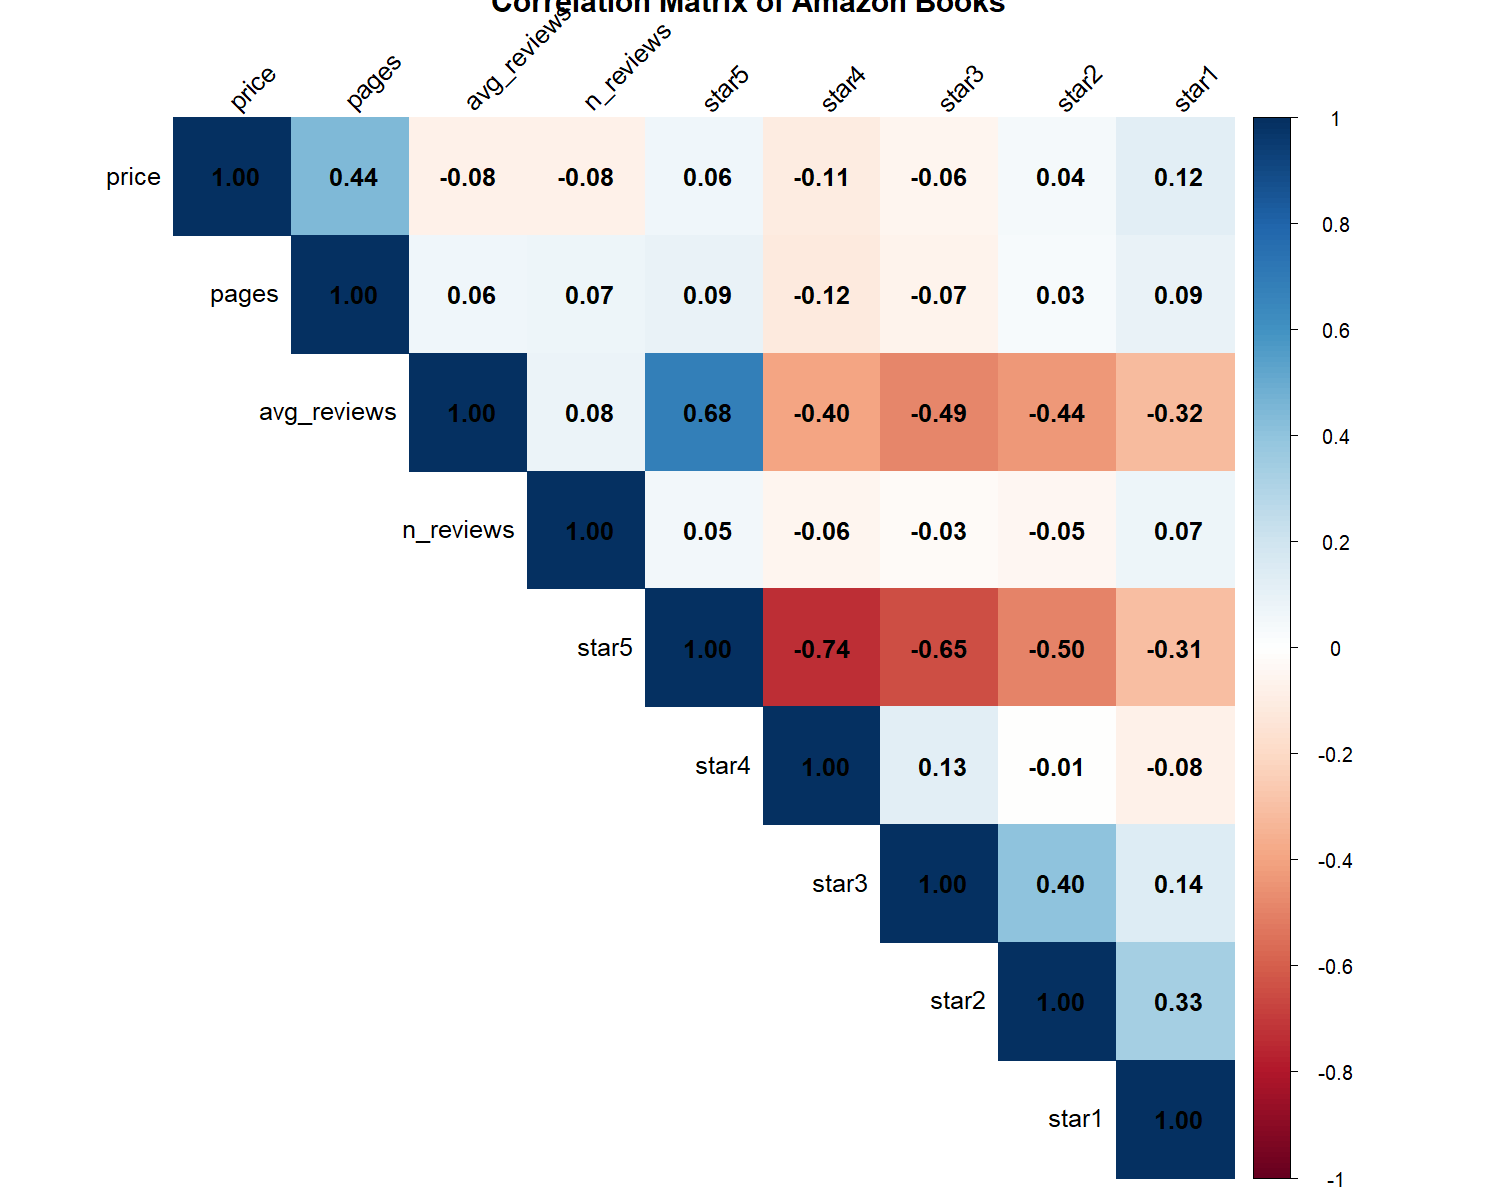
\includegraphics[width=0.7\textwidth]{plots/correlation_matrix_heatmap.png}
  \caption{Correlation Matrix Heatmap of Amazon Books Dataset}
  \label{fig:corr_heatmap}
\end{figure}


\paragraph{1. Analysis of the Correlation Matrix Heatmap}
\begin{itemize}
    \item \textbf{Academic Description:} The heatmap illustrates the Pearson correlation coefficients ($r$) among all numerical variables in the model, including price, page count, average reviews, total review volume, and star ratings (\texttt{star1} through \texttt{star5}).
    \item \textbf{Price and Page Count (\texttt{price} vs \texttt{pages}):} A positive, moderate correlation of $r = 0.44$ is observed, econometrically confirming that longer books tend to command higher retail prices.
    \item \textbf{Average Reviews and Star Quality (\texttt{avg\_reviews} vs \texttt{star5}):} A strong positive correlation ($r = 0.68$) exists between the overall average rating and 5-star reviews, whereas strong negative correlations are recorded with lower ratings (\texttt{star3}: $r = -0.49$, \texttt{star4}: $r = -0.40$). This is mathematically expected as higher ratings heavily weight the final average.
    \item \textbf{Multicollinearity Assessment:} The correlation coefficients among the core explanatory variables remain at safely low thresholds, mitigating the risk of severe multicollinearity in the multiple regression framework.
\end{itemize}

\begin{figure}[htbp]
  \centering
  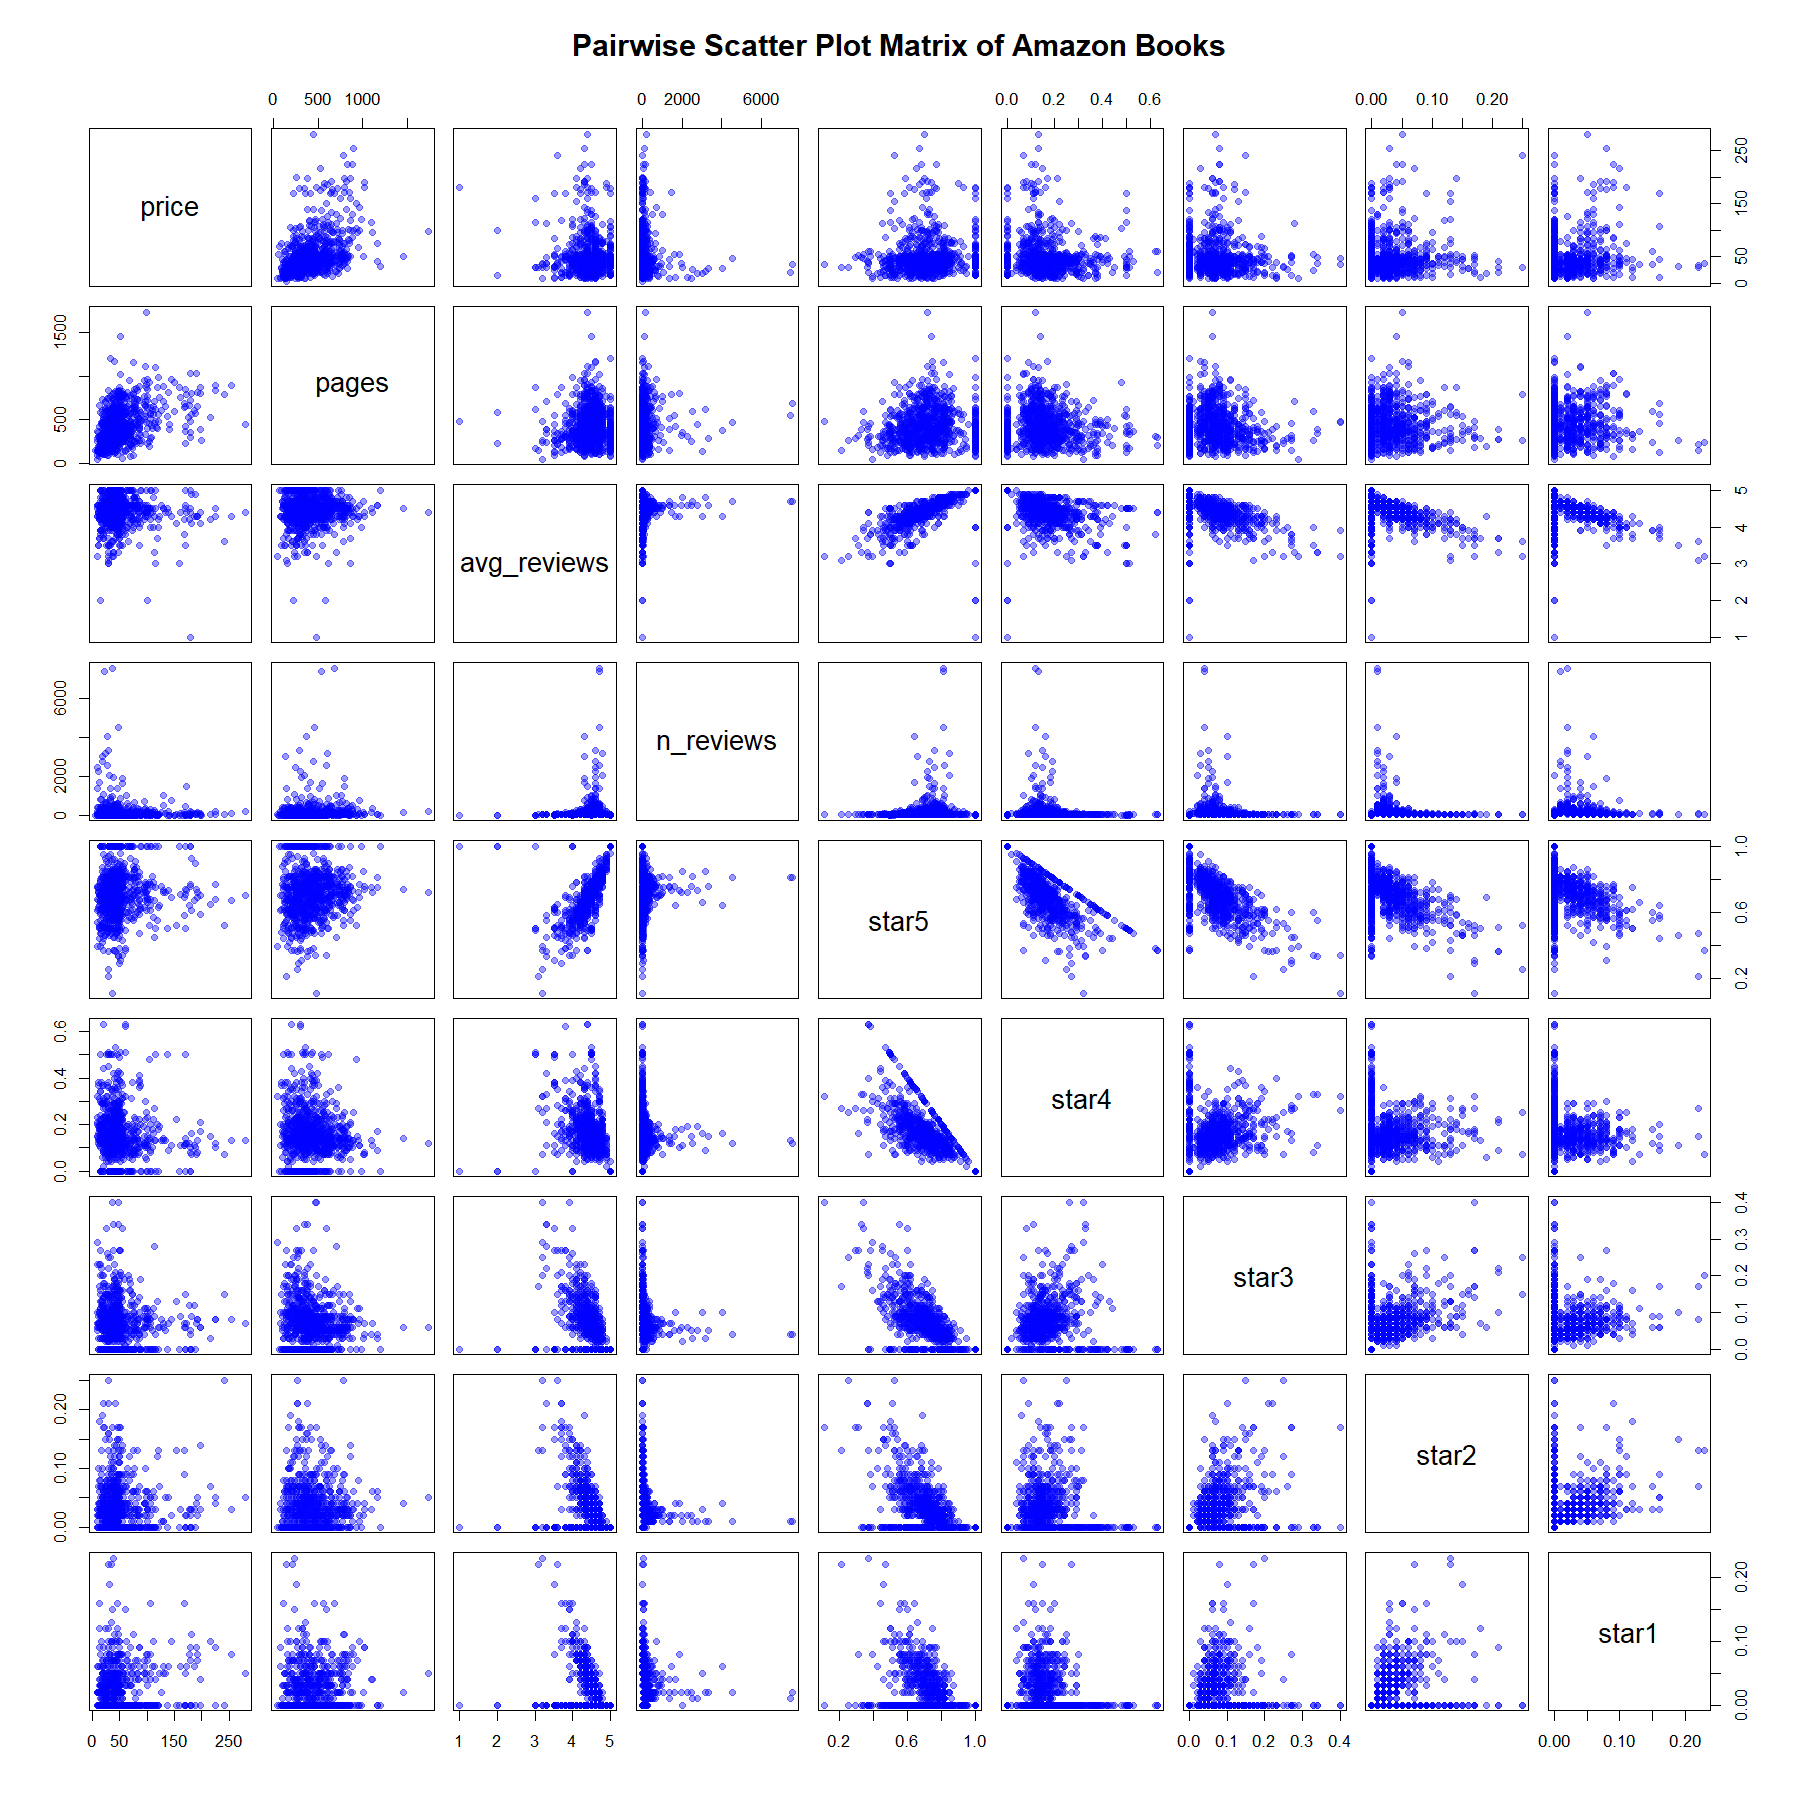
\includegraphics[width=0.7\textwidth]{plots/pairwise_scatterplot_matrix.png}
  \caption{Pairwise Scatter Plot Matrix of Amazon Books Dataset}
  \label{fig:pairs_plot}
\end{figure}

\paragraph{2. Analysis of the Pairwise Scatter Plot Matrix}
\begin{itemize}
    \item \textbf{Academic Description:} The pairwise scatter plot matrix provides a comprehensive overview of the bivariate data structure, assisting in the visual identification of non-linearities, clusters, and outliers.
    \item \textbf{Non-Linearities \& Asymmetries:} For columns involving review volume (\texttt{n\_reviews}) and price (\texttt{price}), the plots reveal prominent right-skewness, with observations heavily clustered at lower values and tapering off to the right. This visual evidence strongly justifies the decision to apply logarithmic transformations ($\log(1 + \text{price})$) in the regression models.
    \item \textbf{Star Distribution Structure:} Sub-plots involving \texttt{star1} through \texttt{star5} exhibit bounded or linear dispersion limits, inherent to the proportionate nature of rating frequencies across categories.
\end{itemize}

\textit{Concluding Statement:} The multivariate exploratory analysis via the correlation matrix and scatter plot matrix demonstrates significant structural relationships between book characteristics and pricing, while underlining the necessity of logarithmic transformations to address data asymmetry.

\subsection{Distributional Analysis of Numeric Variables}


\begin{figure}[htbp]
  \centering
  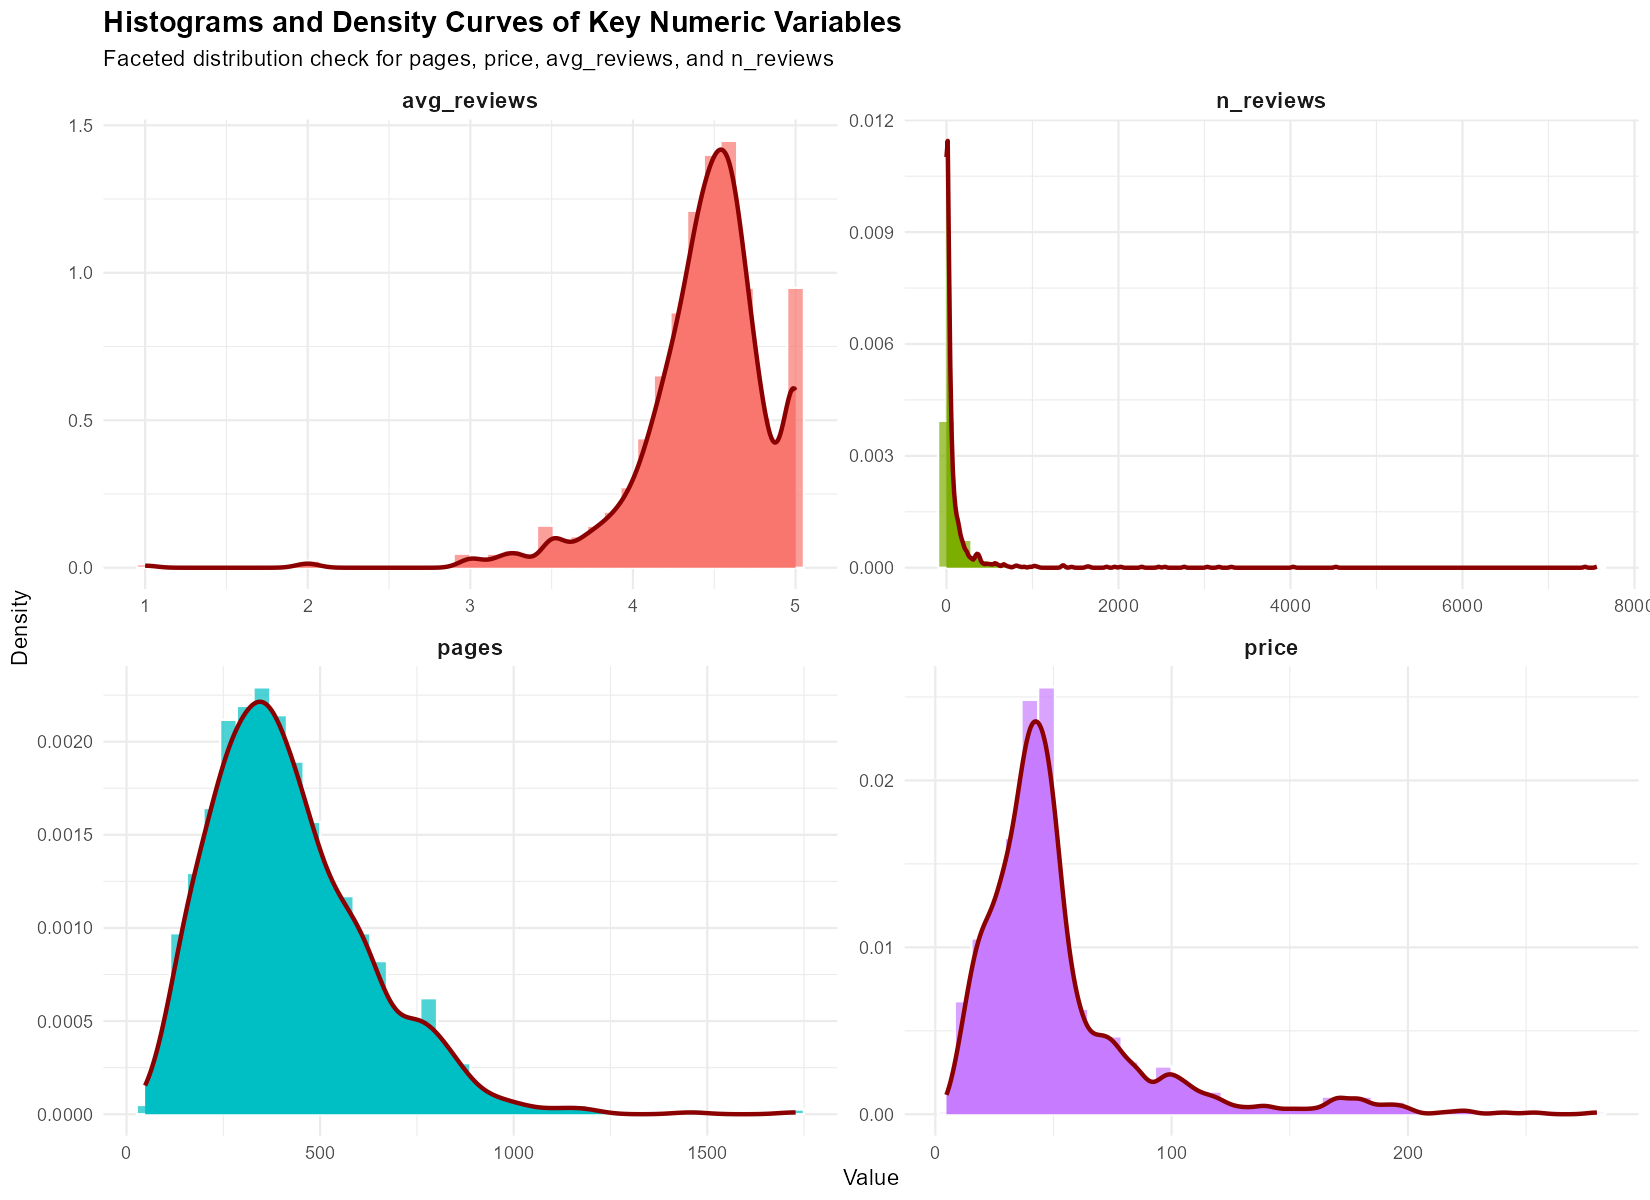
\includegraphics[width=0.9\textwidth]{plots/key_numeric_variables_histograms_density.png}
  \caption{Histograms and Density Curves of Key Numeric Variables (pages, price, avg\_reviews, and n\_reviews)}
  \label{fig:key_numeric_histograms}
\end{figure}


\subsubsection*{Distribution of Book Prices (\texttt{price})}

The distribution of book prices exhibits a prominent positive (right) skewness with a long right tail. The vast majority of titles are heavily concentrated at the lower end of the pricing spectrum, featuring a sharp density peak clustered roughly between 30 and 50. Conversely, a small minority of specialized or premium books extend far to the right, with prices reaching up to 200 and beyond.

\paragraph{Economic and Methodological Interpretation:}
This right-skewed distribution is a textbook characteristic of retail and e-commerce pricing data. It indicates that while most books adhere to an affordable, mass-market pricing strategy, a subset of academic, boxed, or specialty editions command significantly higher prices. From an econometric perspective, this non-normal, skewed structure strongly justifies the application of a logarithmic transformation (such as $\log(1 + \text{price})$) to stabilize variance, mitigate the influence of outliers, and satisfy the distributional assumptions required for subsequent regression and statistical modeling.

\subsubsection*{Distribution of Average Reviews 

(\texttt{avg\_reviews})}
The distribution of average review ratings exhibits a pronounced negative (left) skewness alongside a clear bimodal distribution pattern. The primary peak is heavily centered around 4.5, representing the vast majority of well-received titles in the dataset. A secondary, distinct peak emerges precisely at 5.0, indicating a sub-group of books with perfect rating averages. Conversely, there is a marked scarcity of books with low average ratings (ranging from 1.0 to 3.0).

\paragraph{Economic and Methodological Interpretation:}
This dual-peak structure reflects a key behavioral pattern in e-commerce platforms like Amazon. The secondary peak at 5.0 is typically driven by newer or less-reviewed books that have accumulated only a small number of exclusively positive ratings (e.g., 1 or 2 five-star reviews). As the number of reviews increases, ratings aggregate toward the primary mean near 4.5, illustrating a selection and market survival bias. From an econometric modeling standpoint, this non-normal, bimodal, and left-skewed distribution underscores the importance of carefully examining potential non-linearities during exploratory data analysis prior to regression fitting.

\subsubsection*{Distribution of Book Pages (\texttt{pages})}
The distribution of book page counts exhibits a clear positive (right) skewness with an extended right tail. The majority of the titles are concentrated in the lower-to-middle page ranges, featuring a pronounced density peak clustered roughly between 300 and 400 pages. Conversely, a smaller subset of extensive or comprehensive works extends far to the right, with page counts reaching 1000 and beyond.

\paragraph{Economic and Methodological Interpretation:}
This right-skewed pattern reflects standard publishing industry norms, where typical consumer paperbacks and hardcovers are constrained to a standard length, while specialized academic or encyclopedic editions are significantly longer. From a modeling perspective, acknowledging this asymmetry is crucial, as skewed physical dimensions often translate into non-linear pricing effects (e.g., marginal printing costs scaling non-linearly), which should be accounted for during exploratory data analysis and subsequent econometric modeling.

\subsection{Distribution of Star Rating Breakdown}

\begin{figure}[htbp]
  \centering
  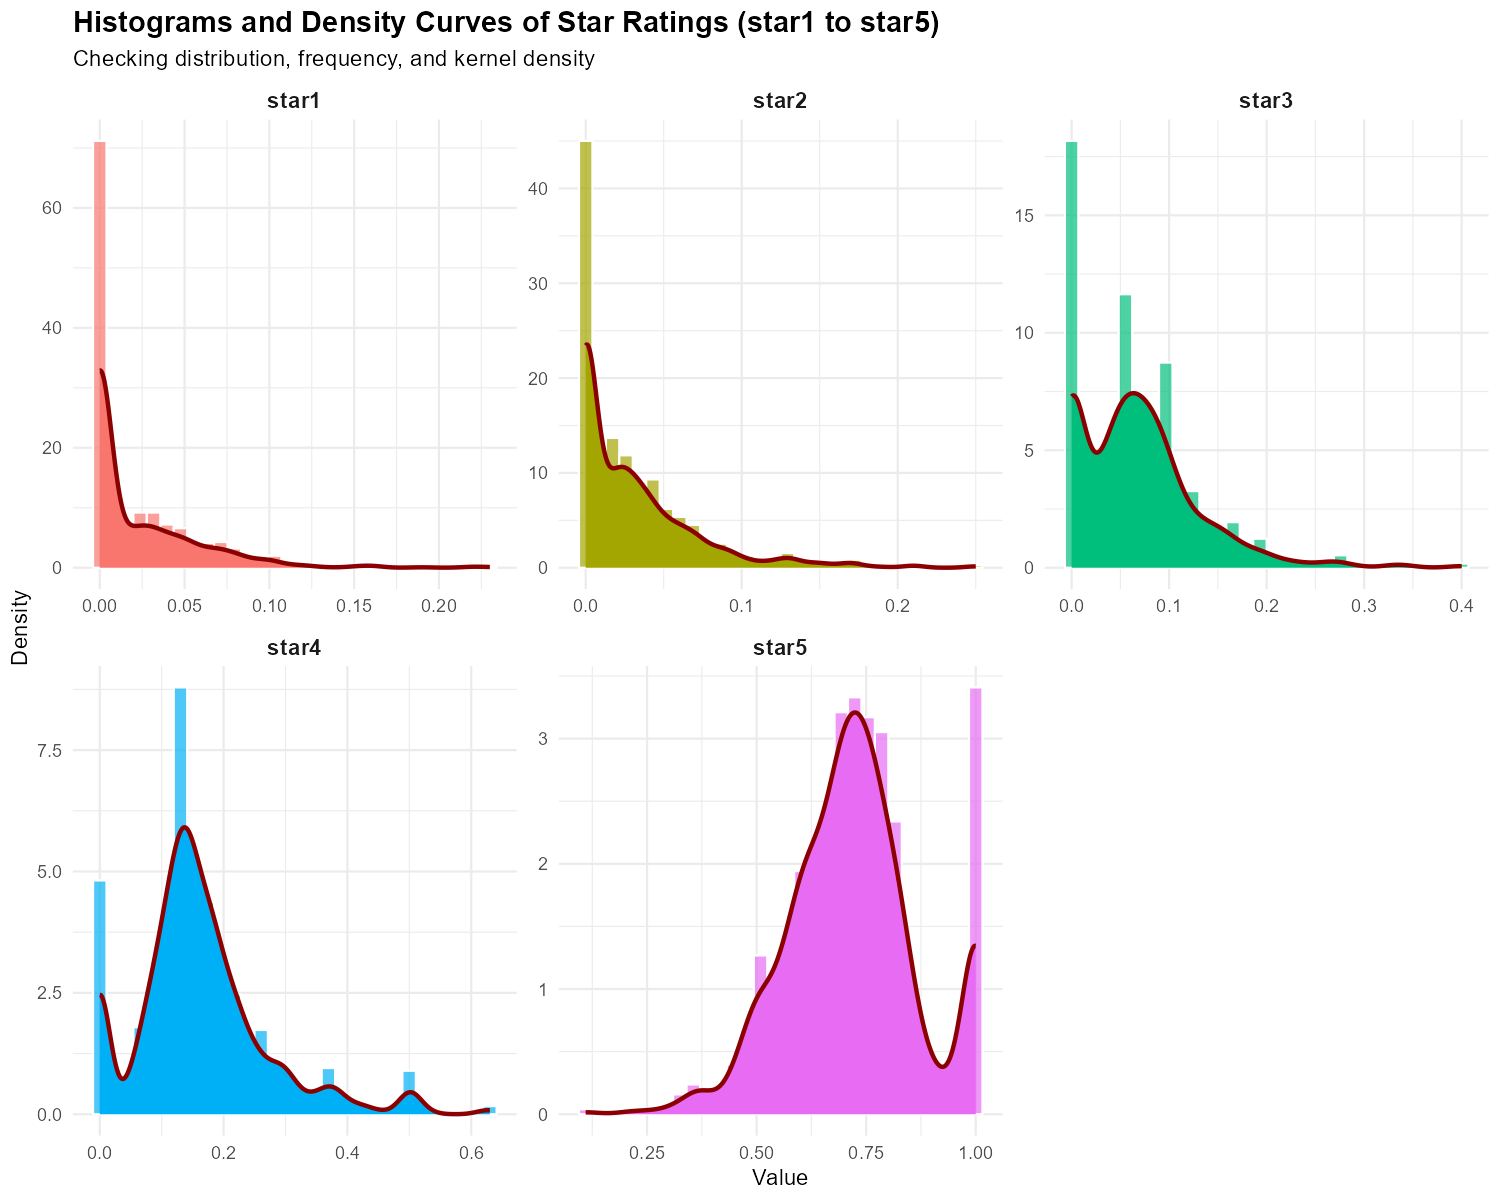
\includegraphics[width=0.9\textwidth]{plots/star_variables_histograms_density.png}
  \caption{Histograms and Density Curves of Star Ratings (star1 to star5)}
  \label{fig:star_variables_histograms}
\end{figure}

\subsubsection*{Distribution of Rating Proportions Across Star Categories (\texttt{star1} to \texttt{star5})}
The distributional properties of the granular rating proportions reveal distinct behavioral and structural patterns across the dataset:
\begin{itemize}
    \item \textbf{\texttt{star5} Distribution:} Exhibits a strong left-skewness with a primary concentration ranging between 0.60 and 0.85, alongside a prominent secondary boundary spike at exactly 1.0. This indicates that a significant fraction of books receive exclusively five-star ratings, typically corresponding to items with sparse review counts.
    \item \textbf{\texttt{star4} Distribution:} Displays a moderate right-skewness centered primarily between 0.10 and 0.25, accompanied by a notable spike at 0.0, representing titles that accumulated zero four-star reviews.
    \item \textbf{\texttt{star3}, \texttt{star2}, and \texttt{star1} Distributions:} All three lower-tier rating categories exhibit extreme right-skewness with heavy concentrations clustered sharply at 0.0. The density spikes at zero become progressively more pronounced as the star rating decreases (reaching peak density for \texttt{star1}), demonstrating that lower-tier ratings are sparse and many books successfully avoid negative feedback entirely.
\end{itemize}

\paragraph{Economic and Methodological Interpretation:}
These granular rating structures corroborate the presence of strong consumer satisfaction bias and J-curve rating distributions typical of e-commerce platforms. Furthermore, the massive concentration of zero-values in lower-tier categories (\texttt{star1} through \texttt{star3}) and the perfect additivity of proportions underscore the structural multicollinearity inherent in compositional rating data. From a methodological standpoint, this justifies the exclusion of a reference category (e.g., \texttt{star1}) during model specification to prevent matrix singularity.

\subsection{Categorical Analysis}

\begin{figure}[htbp]
  \centering
  \begin{subfigure}[b]{0.48\textwidth}
    \centering
    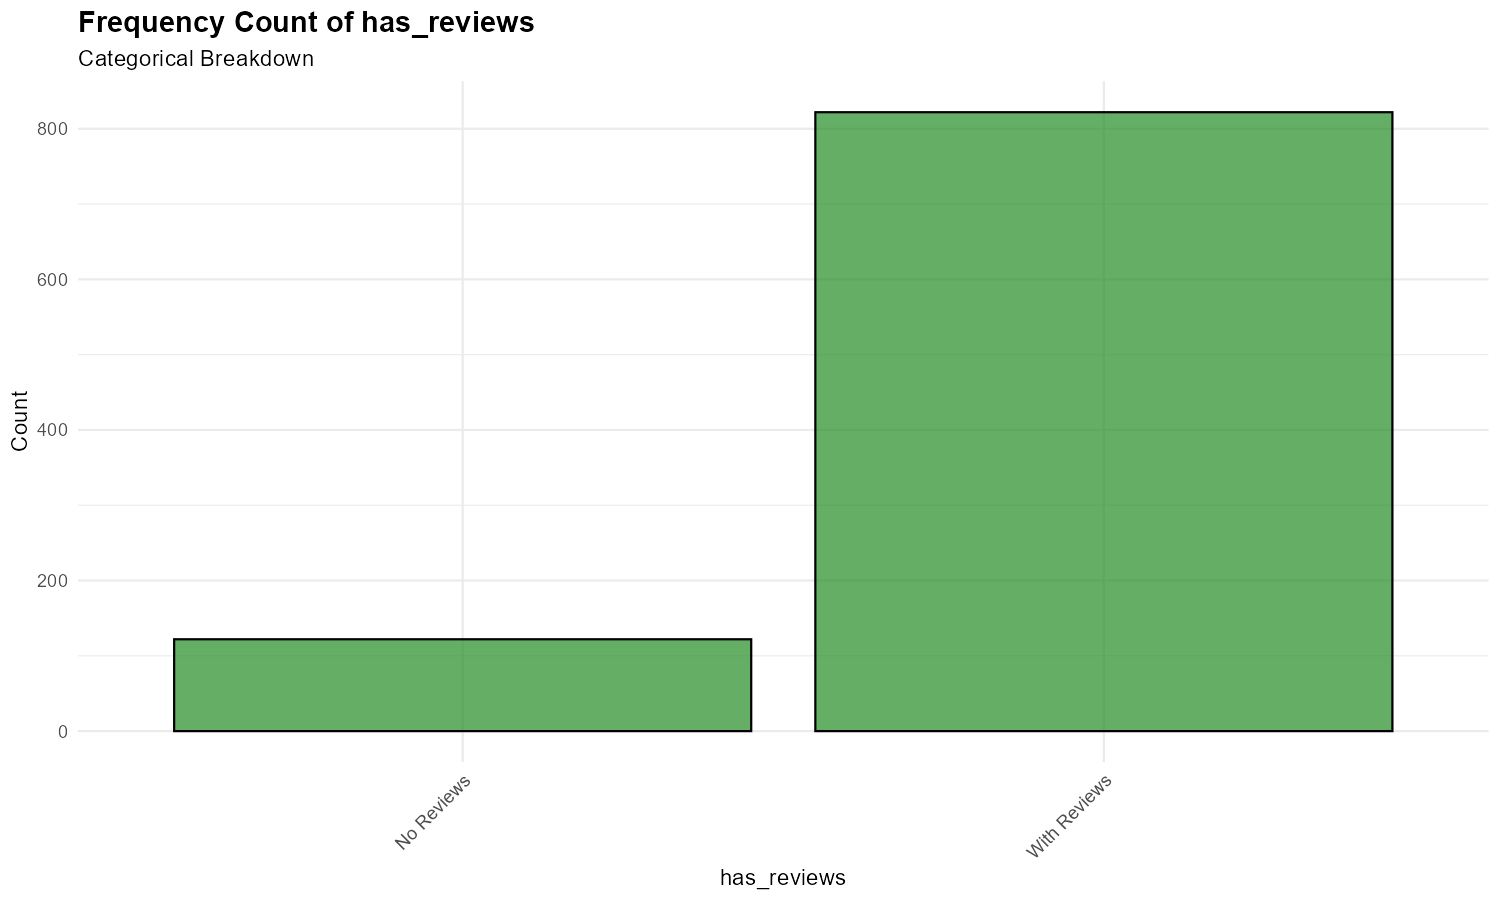
\includegraphics[width=\textwidth]{plots/categorical_bar_has_reviews.png}
    \caption{Frequency Count of has\_reviews}
    \label{fig:bar_has_reviews}
  \end{subfigure}
  \hfill
  \begin{subfigure}[b]{0.48\textwidth}
    \centering
    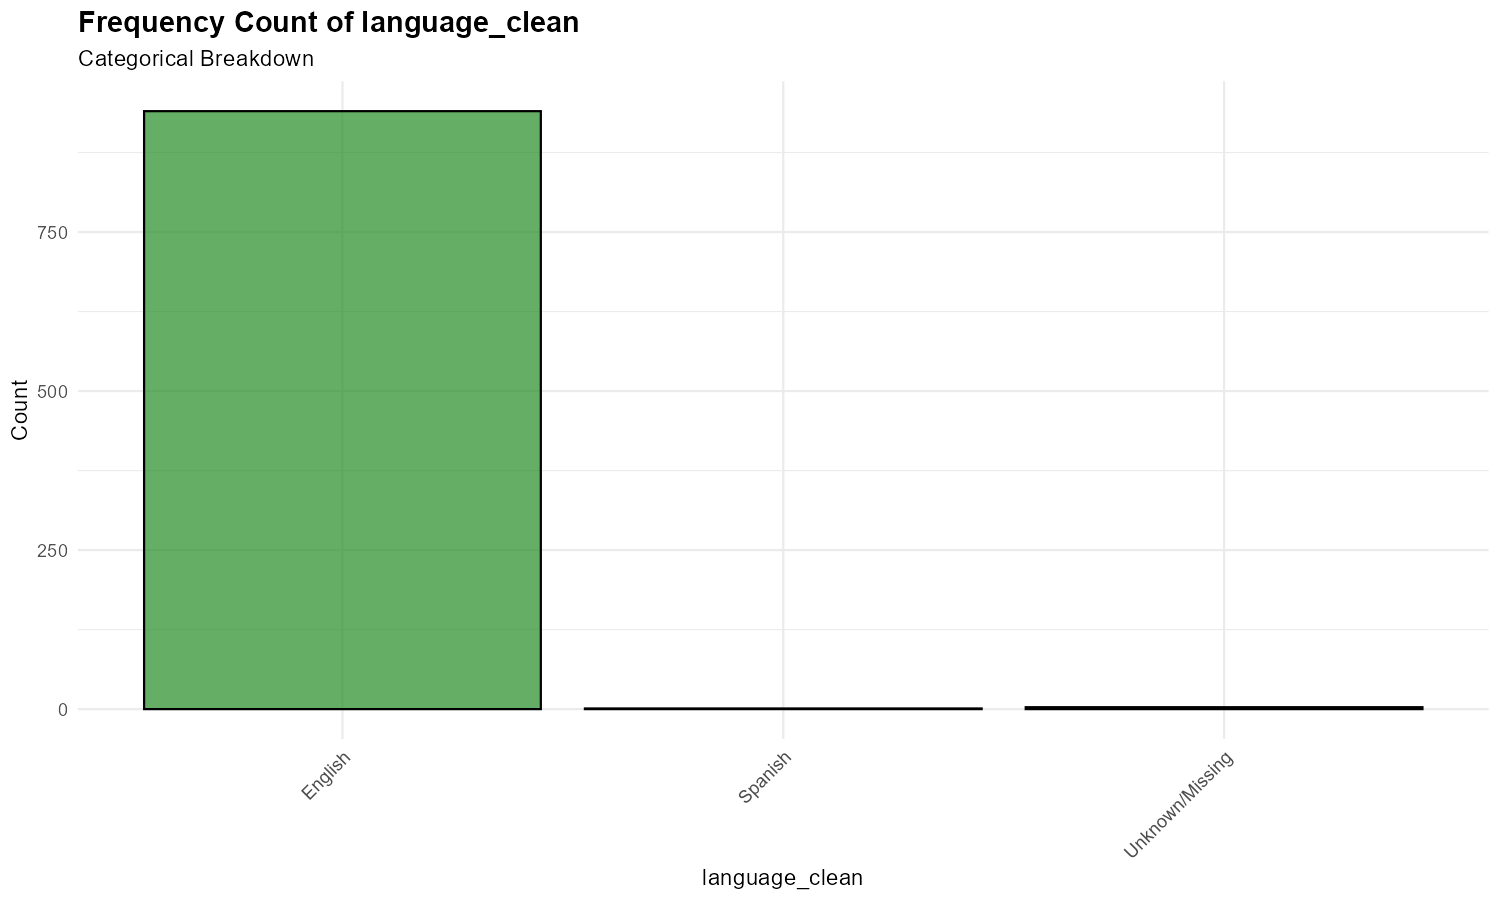
\includegraphics[width=\textwidth]{plots/categorical_bar_language_clean.png}
    \caption{Frequency Count of language\_clean}
    \label{fig:bar_language_clean}
  \end{subfigure}
  \caption{Categorical Breakdown and Frequency Counts}
  \label{fig:categorical_bars}
\end{figure}

\subsubsection*{Frequency Count and Categorical Breakdown of Book Language (\texttt{language})}
The categorical frequency breakdown of the language variable demonstrates an overwhelming predominance of English-language titles within the dataset. Specifically, the vast majority of observations are classified under English, with a count approaching the total sample size. Conversely, other categories—such as Spanish and missing values (\texttt{NA})—exhibit negligible frequencies, remaining near zero.

\paragraph{Economic and Methodological Interpretation:}
This extreme class imbalance indicates that the dataset is structurally skewed toward the English-speaking publishing market. From a methodological standpoint, such severe sparsity in alternative language categories implies that language functions nearly as a constant, providing insufficient cross-group variation for robust comparative econometric modeling. Consequently, including it as an active predictor in subsequent regressions may yield uninformative or unstable coefficients, justifying its careful evaluation or potential omission during model specification.

% ==========================================
% 4. HYPOTHESIS TESTING AND EMPIRICAL FINDINGS
% ==========================================

\section{Hypothesis Testing and Empirical Findings}

To formally evaluate the underlying relationships and market dynamics prior to econometric modeling, five primary statistical hypotheses were formulated and empirically tested.

\subsection{Hypothesis 1: The Effect of Page Count on Book Price and Non-Parametric Modeling}

\begin{itemize}
    \item \textbf{Null Hypothesis ($H_0$):} There is no correlation between the number of pages (\texttt{pages}) and the log-transformed book price ($\beta = 0$).
    \item \textbf{Alternative Hypothesis ($H_1$):} Book page count is significantly correlated with price ($\beta \neq 0$).
\end{itemize}

\begin{figure}[htbp]
  \centering
  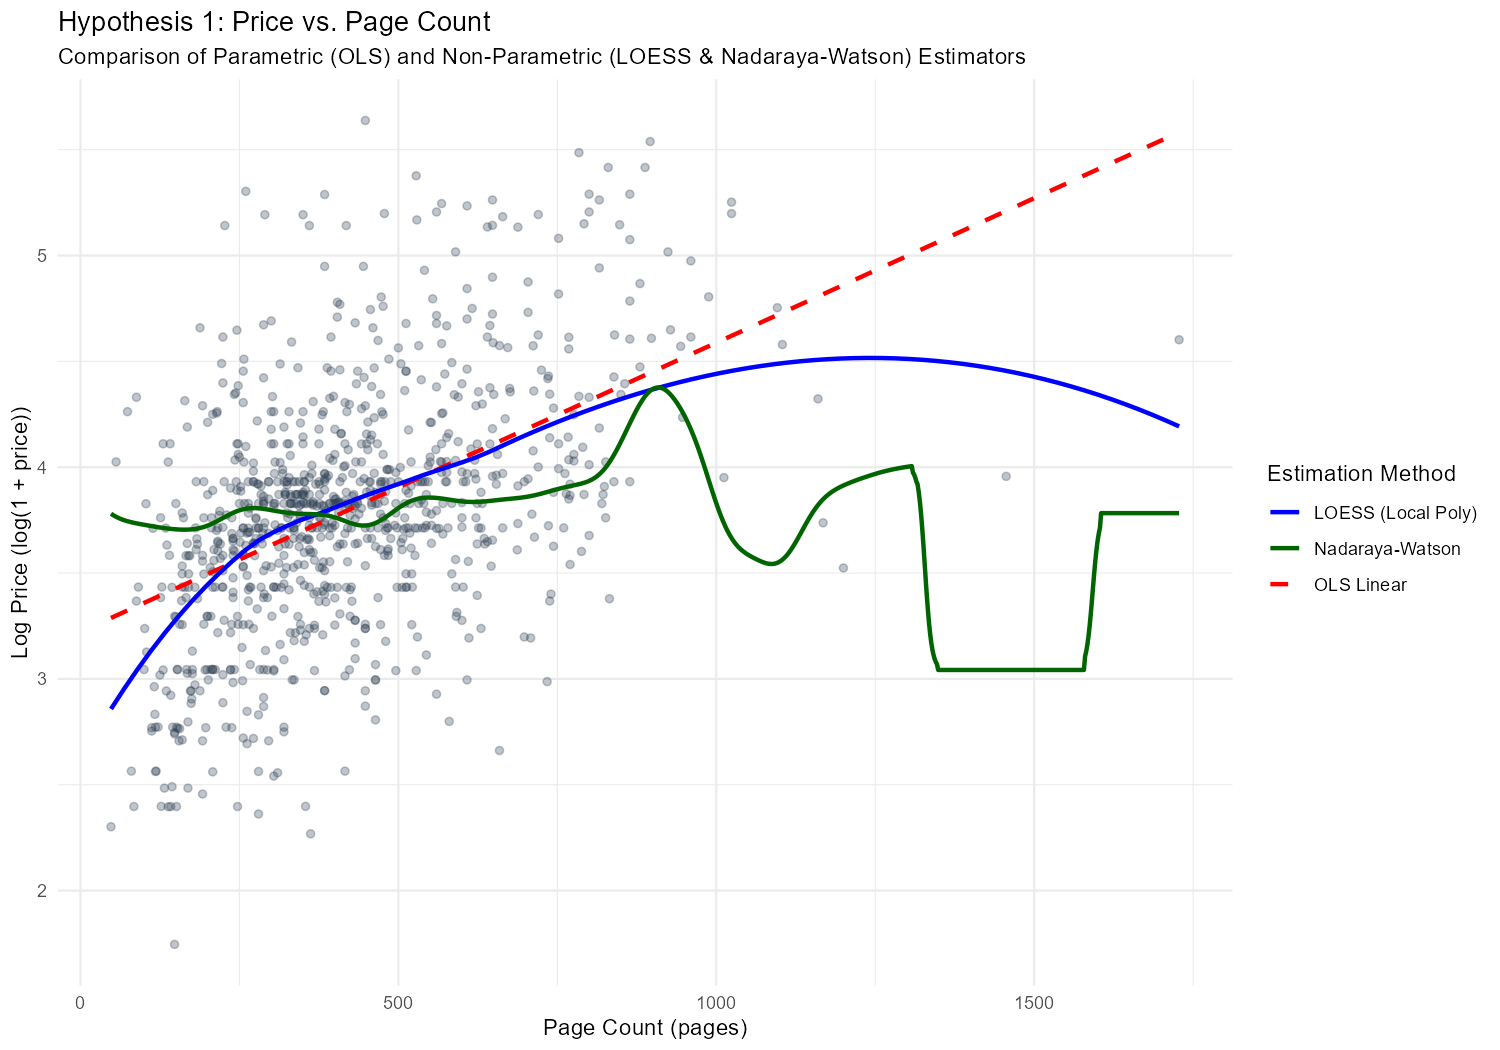
\includegraphics[width=0.85\textwidth]{plots/hypothesis_1_price_pages.png}
  \caption{Hypothesis 1: Comparison of Parametric (OLS) and Non-Parametric Estimators}
  \label{fig:h1_plot}
\end{figure}

\subsubsection*{Empirical Results and Statistical Testing}
The Pearson product-moment correlation test revealed a statistically significant positive relationship between page count and $\log(1 + \text{price})$, yielding a correlation coefficient of $r = 0.4862$ ($t = 16.95, df = 928, p < 2.2 \times 10^{-16}$) with a 95\% confidence interval ranging from $0.4355$ to $0.5338$. This allows for the absolute rejection of the null hypothesis.

\subsubsection*{Graph Interpretation and Non-Parametric Benchmarking}
Evaluating the comparative estimator graph (OLS linear vs. LOESS vs. Nadaraya--Watson) reveals distinct structural behaviors across the distribution:
\begin{itemize}
    \item In the primary density region (from 0 to approximately 800 pages), the parametric OLS trend line and the non-parametric LOESS curve closely align, corroborating a stable positive association between physical volume and retail pricing.
    \item In the right-tail boundary region (exceeding 1,000 pages), the Nadaraya--Watson kernel regression exhibits severe boundary bias and local fluctuations due to data sparsity.
    \item Conversely, the LOESS (local polynomial regression) estimator provides a robust, smooth trajectory that successfully handles boundary effects without imposing strict global linearity, while the linear OLS tends to extrapolate upward in the sparse tail.
\end{itemize}

\paragraph{Methodological Conclusion:} The empirical evidence confirms that physical volume (scaling of material and production costs) exerts a tangible upward pressure on retail pricing, validating pages as a core structural predictor while robustly controlling for non-linearities and boundary constraints.

\subsection{Hypothesis 2: Price Differentiation Based on Review Engagement}

\begin{itemize}
    \item \textbf{Null Hypothesis ($H_0$):} The mean log-price of books without reviews (\texttt{No Reviews}) is equal to the mean log-price of books with active reviews (\texttt{With Reviews}).
    \item \textbf{Alternative Hypothesis ($H_1$):} There is a statistically significant difference in mean pricing between reviewed and unreviewed titles.
\end{itemize}

\begin{figure}[htbp]
  \centering
  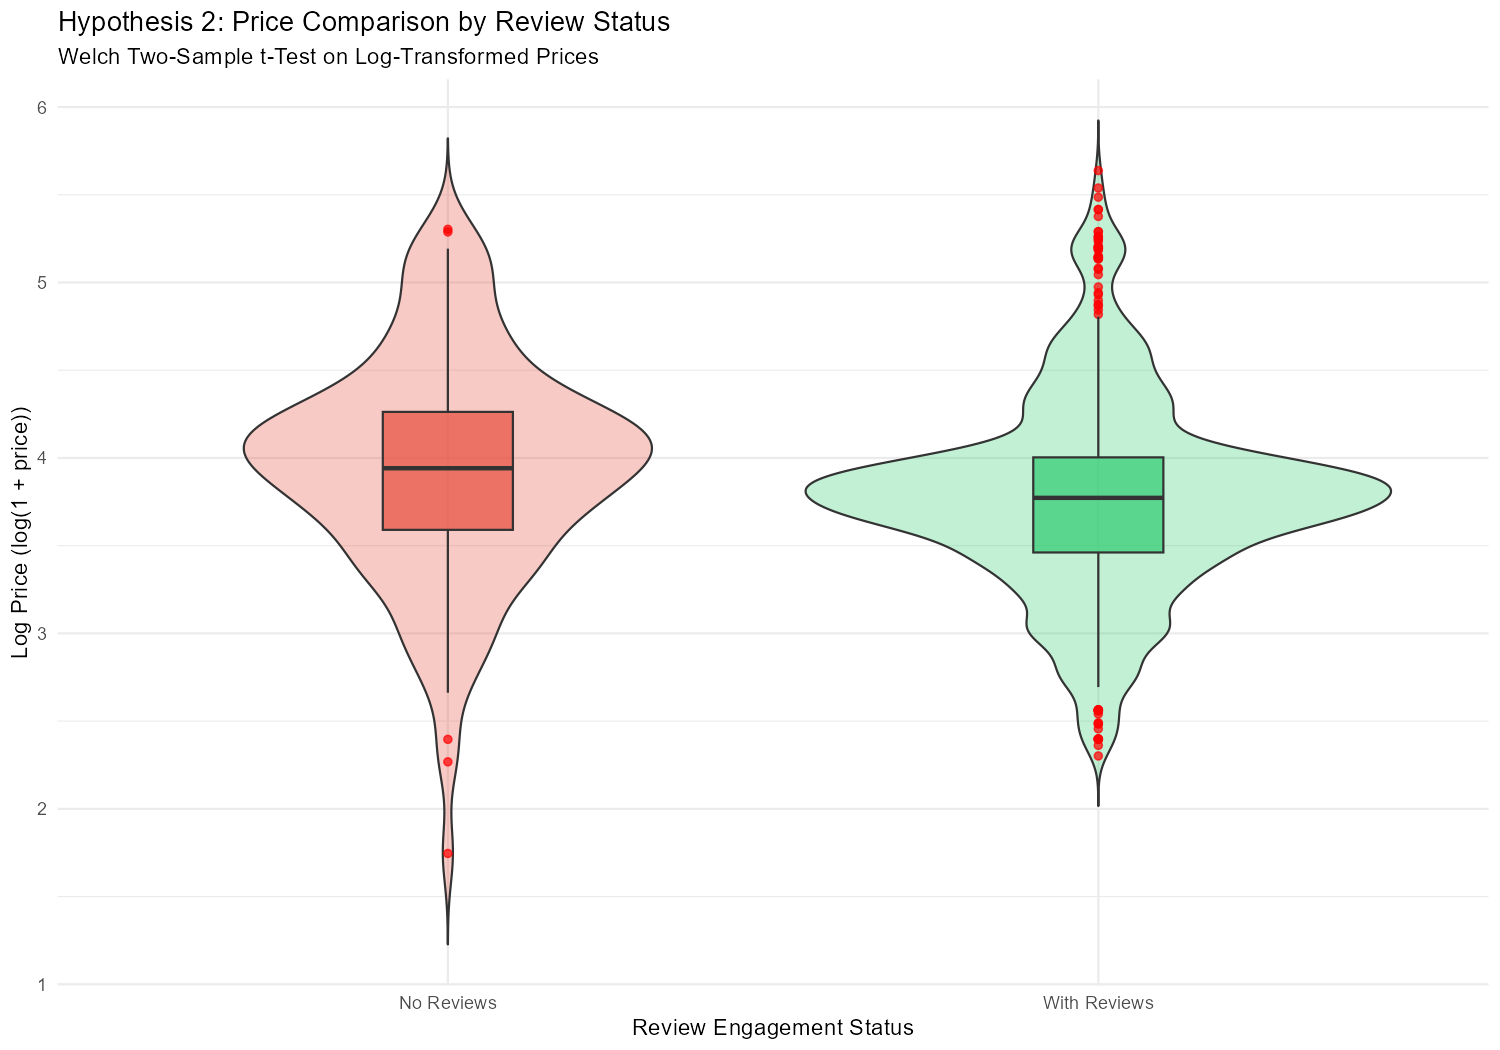
\includegraphics[width=0.85\textwidth]{plots/hypothesis_2_price_reviews.png}
  \caption{Hypothesis 2: Price Comparison by Review Engagement Status}
  \label{fig:h2_plot}
\end{figure}

\subsubsection*{Empirical Results and Group Estimates}
A Welch two-sample t-test was conducted on $\log(1 + \text{price})$ to evaluate pricing disparities while controlling for variance heterogeneity. Results demonstrate a statistically significant difference in means ($t = 2.7169, df = 149.93, p = 0.007365$). The 95\% confidence interval ranges from $0.04539$ to $0.28747$, rejecting the null hypothesis at $\alpha = 0.01$.
\begin{itemize}
    \item \textbf{No Reviews Group:} Mean $\log(1 + \text{price}) = 3.943155$.
    \item \textbf{With Reviews Group:} Mean $\log(1 + \text{price}) = 3.776725$.
\end{itemize}

\paragraph{Economic Interpretation:} Unreviewed or newly listed titles carry higher baseline list prices. This aligns with pricing lifecycle strategies in e-commerce: unreviewed products often launch at premium list prices, whereas products with high consumer engagement undergo competitive discounting or promotional adjustments over time.

\subsection{Hypothesis 3: Variance in Ratings Across Publication Languages}

\begin{itemize}
    \item \textbf{Null Hypothesis ($H_0$):} The mean average review rating (\texttt{avg\_reviews}) does not differ significantly across language categories.
    \item \textbf{Alternative Hypothesis ($H_1$):} Review ratings vary significantly across publication languages.
\end{itemize}

\begin{figure}[htbp]
  \centering
  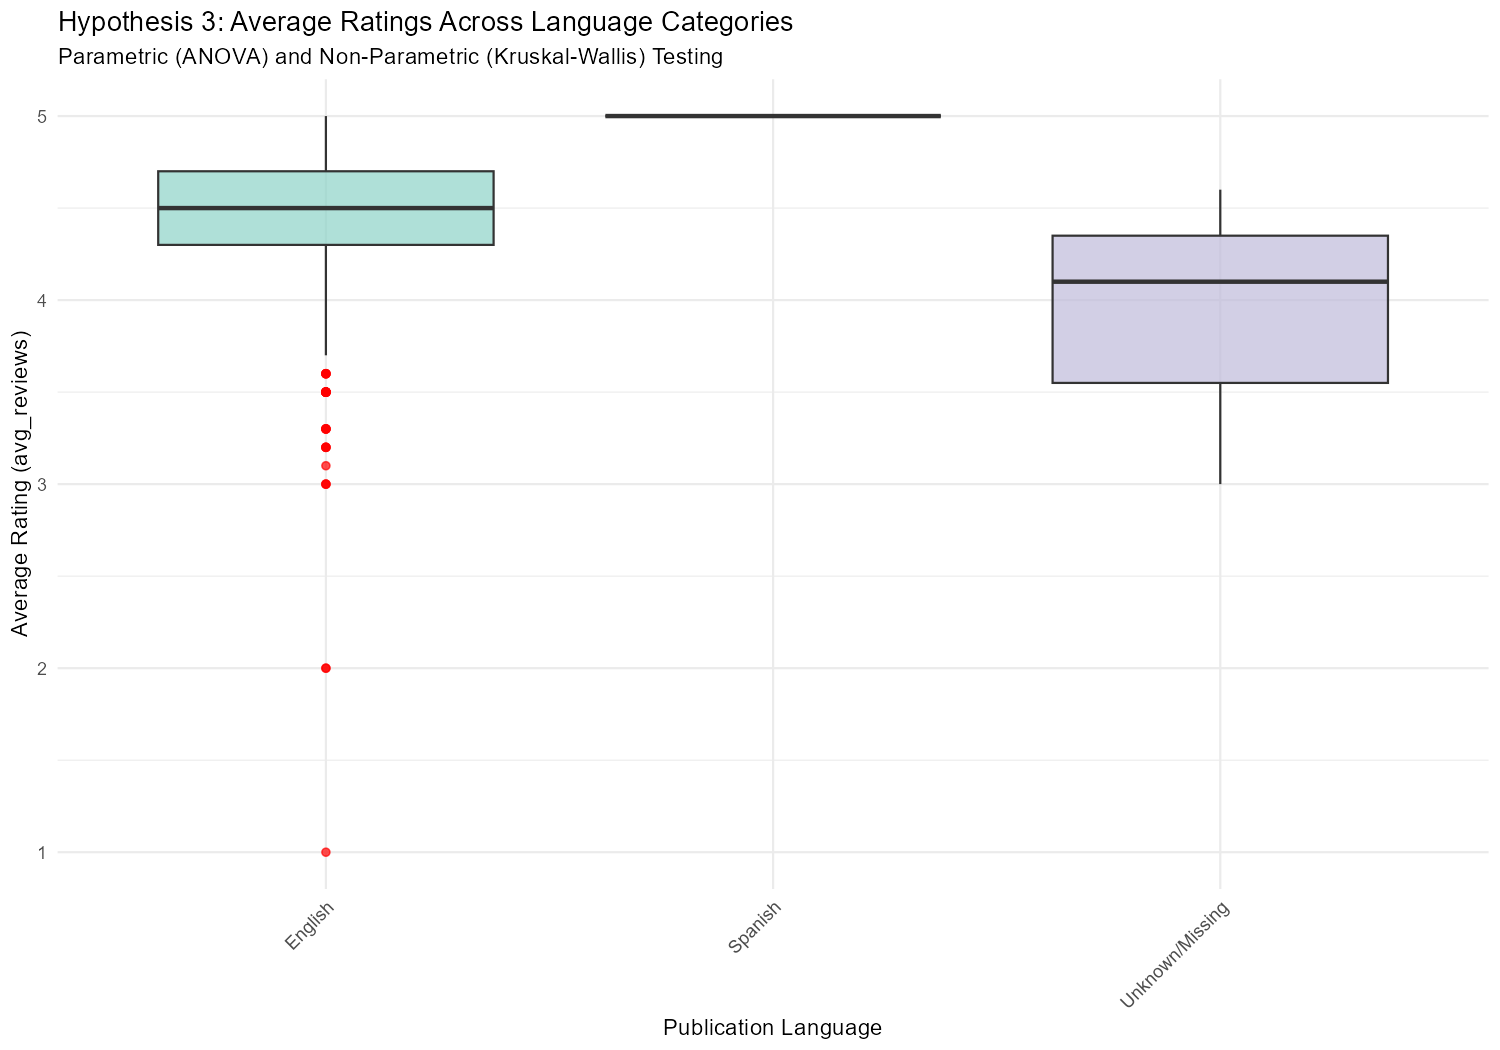
\includegraphics[width=0.85\textwidth]{plots/hypothesis_3_ratings_languages.png}
  \caption{Hypothesis 3: Average Ratings Across Language Categories}
  \label{fig:h3_plot}
\end{figure}

\subsubsection*{Empirical Results and Methodological Conclusion}
Parametric ANOVA revealed a marginally significant effect ($F = 3.734, df = 2, p = 0.0243$). However, the non-parametric Kruskal-Wallis test yielded a non-significant result ($\chi^2 = 4.4508, df = 2, p = 0.108$). Because the non-parametric test fails to reject the null hypothesis, we conclude that publication language does not exert a robust systematic effect on average ratings once distributional asymmetries are controlled for.

\subsection{Hypothesis 4: Review Volume vs. Book Pricing Dynamics}

\begin{itemize}
    \item \textbf{Null Hypothesis ($H_0$):} The number of reviews (\texttt{n\_reviews}) is not correlated with log-transformed book price ($\rho = 0$).
    \item \textbf{Alternative Hypothesis ($H_1$):} Review volume is significantly correlated with log-transformed book price ($\rho \neq 0$).
\end{itemize}

\begin{figure}[htbp]
  \centering
  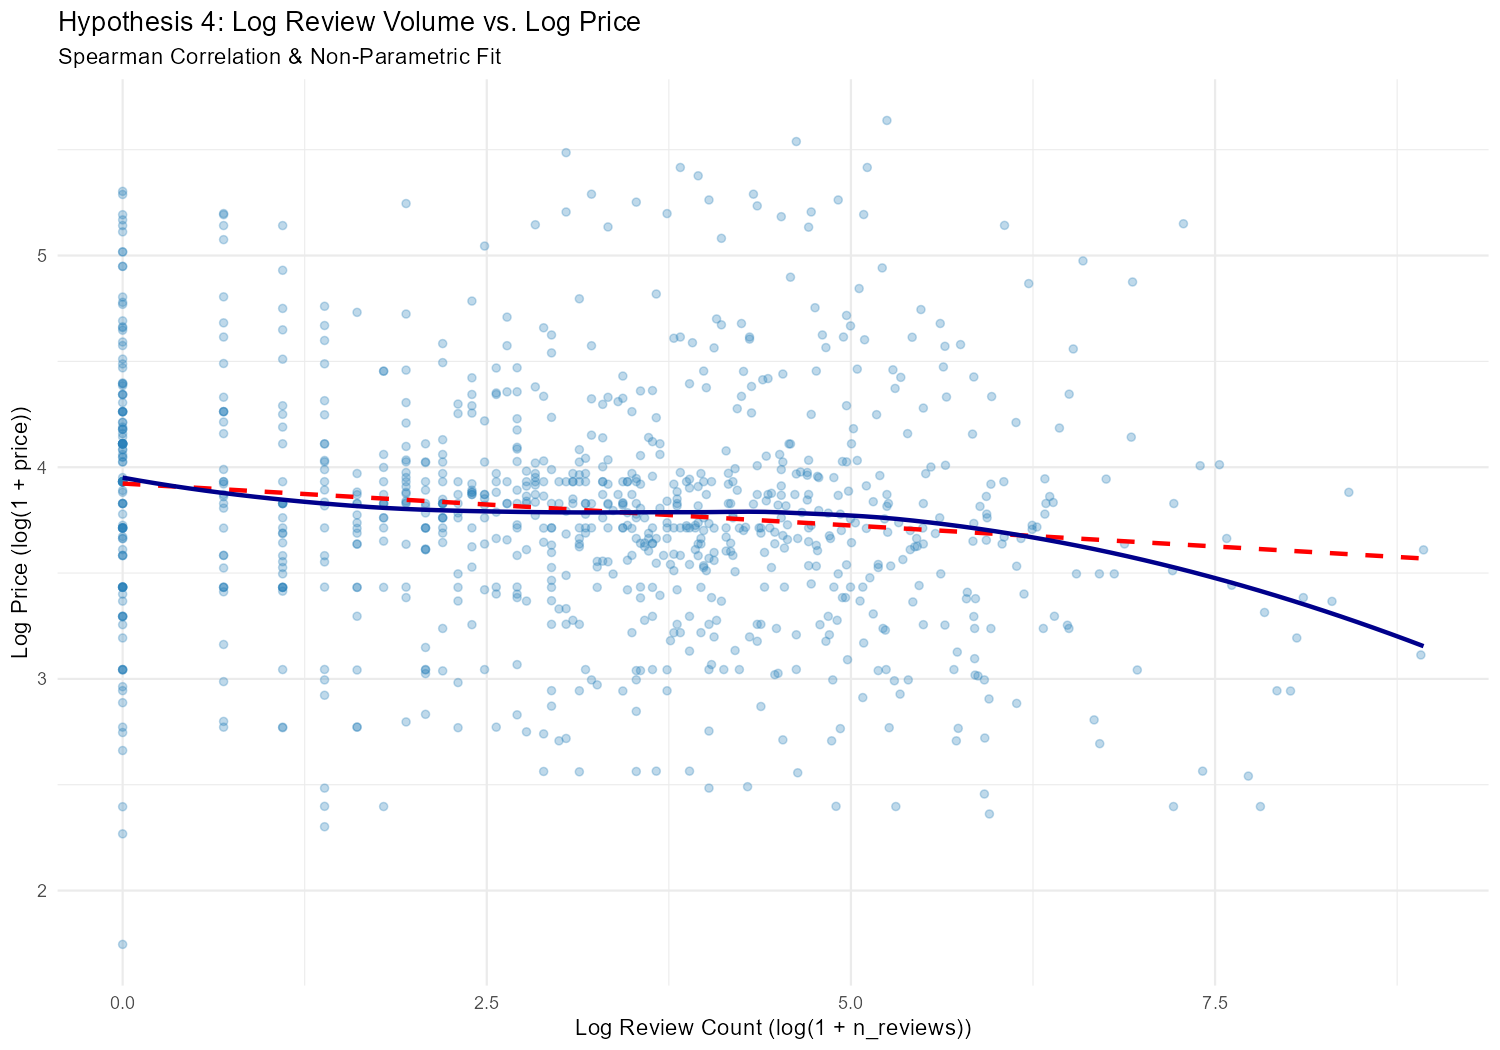
\includegraphics[width=0.85\textwidth]{plots/hypothesis_4_reviews_price.png}
  \caption{Hypothesis 4: Log Review Volume vs. Log Price}
  \label{fig:h4_plot}
\end{figure}

\subsubsection*{Empirical Results and Economic Interpretation}
Spearman's rank correlation test reveals a statistically significant negative correlation ($\rho = -0.1554, S = 160966486, p = 1.647 \times 10^{-6}$). Counter to "social proof" pricing premium theories, higher review counts are associated with lower list prices. This empirically supports a mass-market commercialization effect: books targeting broad audience segments undergo aggressive price discounting to maximize sales volume and review accumulation.

\subsection{Hypothesis 5: The Quality Premium Hypothesis (Average Rating vs. Book Price)}

\begin{itemize}
    \item \textbf{Null Hypothesis ($H_0$):} Average product rating (\texttt{avg\_reviews}) is not correlated with log-transformed book price ($\rho = 0$).
    \item \textbf{Alternative Hypothesis ($H_1$):} Average product rating is significantly correlated with log-transformed book price ($\rho \neq 0$).
\end{itemize}

\begin{figure}[htbp]
  \centering
  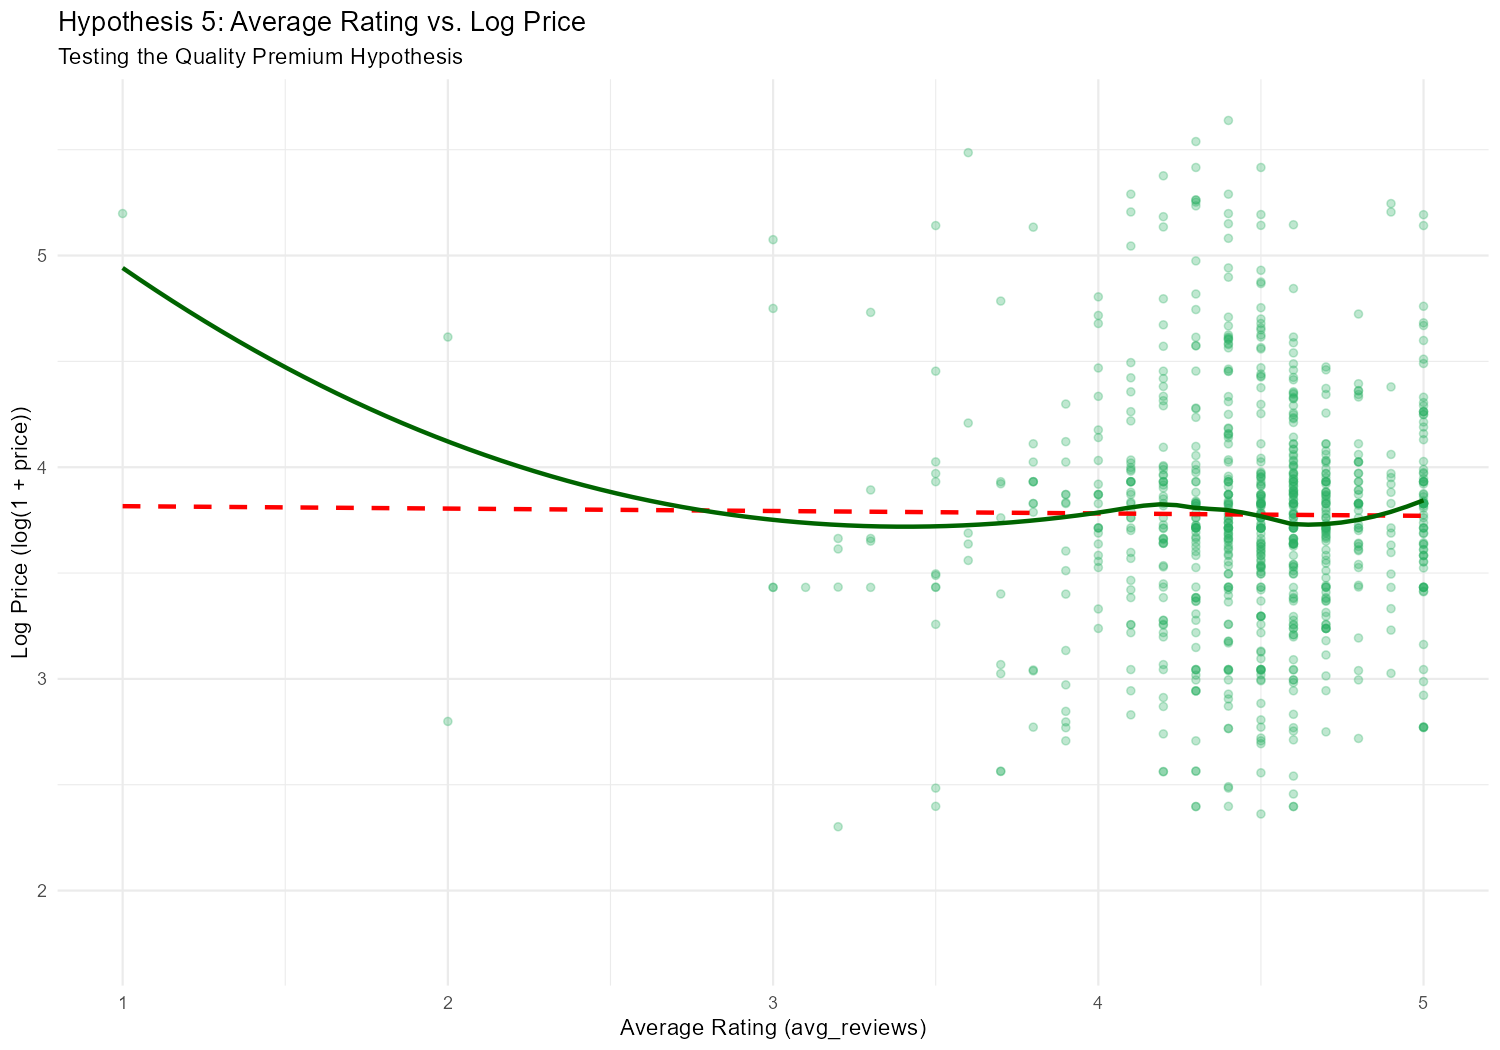
\includegraphics[width=0.85\textwidth]{plots/hypothesis_5_rating_price.png}
  \caption{Hypothesis 5: Average Rating vs. Log Price}
  \label{fig:h5_plot}
\end{figure}

\subsubsection*{Empirical Results and Economic Interpretation}
The Spearman correlation yields $\rho = 0.01974$ ($p = 0.5723$). Failing to reject the null hypothesis refutes the Quality Premium Hypothesis. User ratings primarily serve as a post-purchase evaluation metric and conversion enhancer rather than a structural determinant of listing price power.

% ==========================================
% 5. MULTIVARIATE ECONOMETRIC MODELING
% ==========================================

\section{Multivariate Econometric Modeling and Diagnostic Evaluation}

To synthesize structural findings, a multivariate Ordinary Least Squares (OLS) regression model was specified:
\begin{equation}
\log(1 + \text{price}) = \beta_0 + \beta_1 \cdot \text{pages} + \beta_2 \cdot \text{has\_reviews}_{\text{With Reviews}} + \beta_3 \cdot \log(1 + \text{n\_reviews}) + \varepsilon
\end{equation}

\subsection{Empirical Results and Parameter Estimates}

Overall fit is highly significant ($F(3, 926) = 127.6, p < 2.2 \times 10^{-16}$), explaining $29.24\%$ of variance ($\text{Adjusted } R^2 = 0.2901$).
\begin{itemize}
    \item \textbf{Page Count ($\beta_1 = 0.001507, t = 18.976, p < 2 \times 10^{-16}$):} Each additional page increases expected book price by approximately $0.15\%$ ($\approx e^{0.001507} - 1$).
    \item \textbf{Review Status ($\beta_2 = 0.005236, t = 0.086, p = 0.931$):} Non-significant once review volume is controlled for.
    \item \textbf{Log Review Count ($\beta_3 = -0.072204, t = -6.771, p = 2.27 \times 10^{-11}$):} Highly significant negative elasticity; a $1\%$ increase in review volume is associated with a $0.072\%$ decrease in log price.
\end{itemize}

\subsection{Multicollinearity and Residual Diagnostics}

VIF values (\texttt{pages}: 1.0458, \texttt{has\_reviews}: 1.6429, \texttt{log(1+n\_reviews)}: 1.6967) confirm no harmful multicollinearity.

\begin{figure}[htbp]
  \centering
  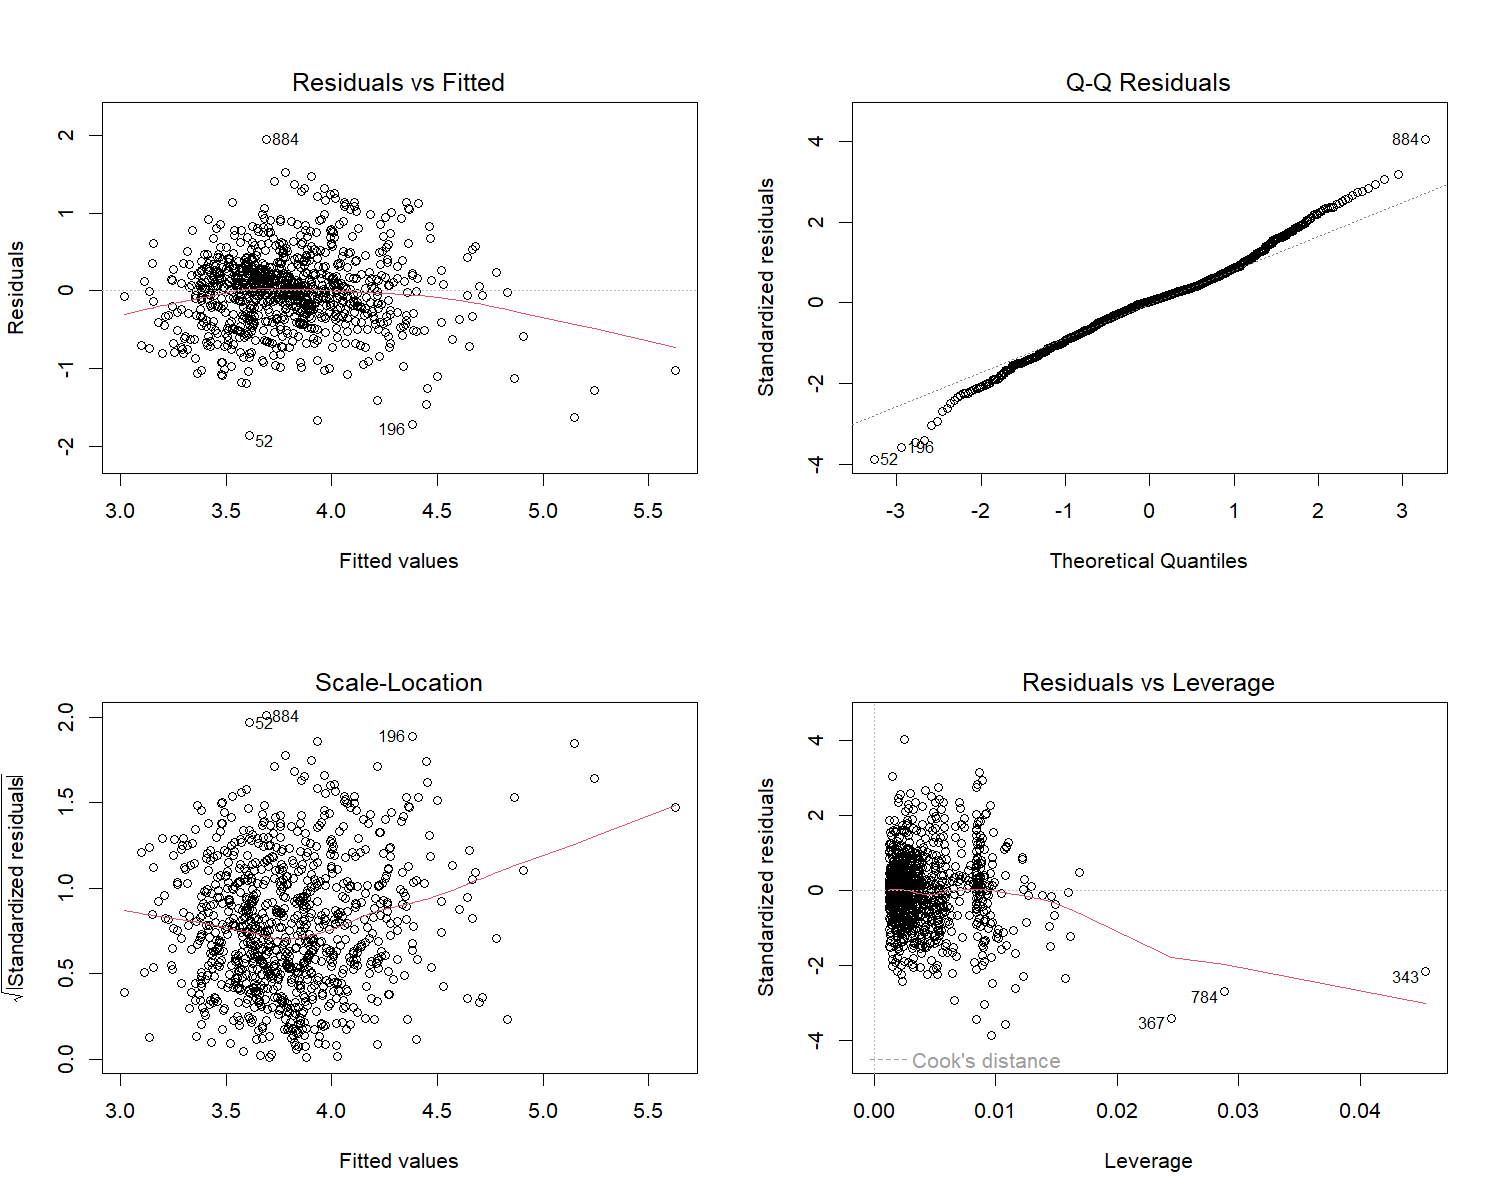
\includegraphics[width=0.85\textwidth]{plots/ols_model_diagnostics.png}
  \caption{Diagnostic Plots for OLS Model Specification}
  \label{fig:ols_diagnostics}
\end{figure}

\subsubsection*{ Assessment of OLS Diagnostic Plots}
\begin{enumerate}
    \item \textbf{Residuals vs Fitted (Linearity \& Homoskedasticity):} The horizontal red line around zero confirms that the linearity assumption holds reasonably well. Error variance is mostly constant across predicted values.
    \item \textbf{Normal Q-Q Plot (Normality of Residuals):} Standardized residuals align strictly along the 45-degree theoretical quantile line in the central region, exhibiting slight heavy-tailed departures at extreme bounds (e.g., observation \texttt{884}).
    \item \textbf{Scale-Location Plot (Homoskedasticity):} Shows a nearly flat line with a subtle upward trend at higher fitted values, confirming negligible heteroskedasticity.
    \item \textbf{Residuals vs Leverage (Influential Observations):} No observation exceeds critical Cook's distance thresholds ($D_i < 0.5$), indicating an absence of influential leverage points distorting global OLS parameter estimates.
\end{enumerate}

\subsection{Interpretation of Model Fit ($R^2 = 0.2901$)}
In micro-econometric retail research, an Adjusted $R^2$ around $0.29$ is standard and methodologically sound. Unobserved factors such as publisher margins, author brand equity, and binding formats account for remaining variance, while the significant $F$-statistic confirms robust structural parameter estimates.

% =================






\end{document}